\documentclass[a4paper,11pt,oneside]{book}
\usepackage[latin1]{inputenc}
\usepackage[english]{babel}
\usepackage{amsfonts}
\usepackage{amsmath}
\usepackage{amssymb,amsmath,color}
\usepackage{cite}
\usepackage{graphicx}
\usepackage{float}
\usepackage{ragged2e}
\usepackage{geometry}         % Customize page layout
\geometry{
    left=3cm,
    right=3cm,
    top=3cm,
    bottom=3cm,
}

\begin{document}
\pagestyle{myheadings}

%%%%%%%%%%% Cover %%%%%%%%%%%
\thispagestyle{empty}                                                 
\begin{center}                                                            
    \vspace{5mm}
    {\LARGE UNIVERSIT\`A DI BOLOGNA}
    \vspace{5mm}
\end{center}
\begin{center}
 % 
\includegraphics[scale=.27]{figs/logo_unibo}
\end{center}
\begin{center}
      \vspace{5mm}
      {\LARGE School of Engineering} \\
        \vspace{3mm}
      {\Large Master Degree in Automation Engineering} \\
      \vspace{20mm}
      {\LARGE Optimal Control} \\
      \vspace{5mm}
      {\Large\textbf{Course Project 1 - Group 3}} \\
      \vspace{3mm}{\Large\textbf{Flexible Robotic Arm Assignment}}                  
      \vspace{15mm}
\end{center}
\begin{flushleft}                                                                              
     {\large Professor: \textbf{Giuseppe Notarstefano}}   
      
\end{flushleft}
\begin{flushleft}                                                                              
     {\large Tutor: \textbf{Marco Falotico}} 
     \vspace{13mm}
\end{flushleft}
\begin{flushright}
      {\large Students:}
\end{flushright}        %capoverso allineato a destra
\begin{flushright}
      {\large Alessandro Letti}
\end{flushright}        %capoverso allineato a destra
\begin{flushright}
      {\large Vincenzo Lombardi}
\end{flushright}        %capoverso allineato a destra
\begin{flushright}
      {\large Giorgia Bettini}
\end{flushright}        %capoverso allineato a destra

\begin{center}
\vfill
      {\large Academic year \@2024/2025} \\
\end{center}



\newpage
\thispagestyle{empty}

%%%%%%%%%%% Abstract %%%%%%%%%%%%
\begin{center}
\chapter*{}
{\Huge \textbf{Abstract}}\\
\vspace{15mm}
\end{center}
\begin{justify}
    The assignment we developed over the past few weeks focuses on designing an optimal control strategy for a flexible robotic arm. The system we worked with is defined as a planar two-link structure where only the first joint is actuated. The key tasks to which we dedicated are trajectory generation between certain pre-defined equilibria using Newton\textquotesingle s-like optimization algorithms and tracking of them using Linear Quadratic Regulator (LQR) and/or Model Predictive Control (MPC) strategies. Once the control algorithms were implemented, their performances were evaluated under perturbed initial conditions and in the presence of measurement noise. We were able to observe the results of our work through plots and animations, which provided insights into system behavior, trajectory adherence, and controller robustness.
\end{justify}

\tableofcontents \thispagestyle{empty}
% \listoffigures\thispagestyle{empty}

%%%%%%%%%% Introduction %%%%%%%%%%
\chapter*{Introduction}
\begin{flushleft}
    {During the implementation of the project, we followed six different assigned tasks:}
\end{flushleft}
\begin{itemize}
    \item \textbf{Task 0 - Problem Setup:} discretize the dynamics, write the discrete-time state-space equations and code the related dynamic function.
    
    \item \textbf{Task 1 - Trajectory generation (I):} compute two equilibria for your system and define a reference curve between the two. Compute the optimal transition to move from one equilibrium to another exploiting the Newton\textquotesingle s-like algorithm (in closed-loop version) for optimal control.
    
    \item \textbf{Task 2 - Trajectory generation (II):} generate a desired (smooth) state-input curve and perform the trajectory generation task (Task 1) on this new desired curve.
    
    \item \textbf{Task 3 - Trajectory tracking via LQR:} linearizing the robot dynamics about the generated trajectory (\(x_{\text{gen}}, u_{\text{gen}}\)) computed in Task 2, exploit the LQR algorithm to define the optimal feedback controller to track this reference trajectory. The cost matrices of the regulator are a degree-of-freedom we had.
    
    \item \textbf{Task 4 - Trajectory tracking via MPC:} linearizing the robot dynamics about the trajectory (\(x_{\text{gen}}, u_{\text{gen}}\)) computed in Task 2, exploit an MPC algorithm to track this reference trajectory.
    
    \item \textbf{Task 5 - Animation:} produce a simple animation of the robot executing Task 3.
\end{itemize}
\addcontentsline{toc}{chapter}{Introduction}




%%%%%%%%%% Chapters %%%%%%%%%%
\chapter{Task 0 - Problem setup}
\section{System definition}
\begin{flushleft}
    {The system is such that it can be modeled as a flexible arm model as shown in Figure 1.1.}
\end{flushleft}
\begin{figure}[H]
    \centering
    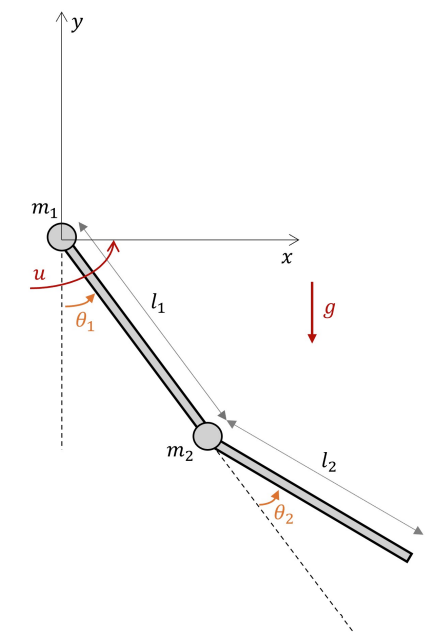
\includegraphics[width=0.3\linewidth]{image.png}
    \caption{flexible arm}
    \label{fig:enter-label}
\end{figure}
\begin{flushleft}
    {The state space consists in: \[x = [\theta_1, \theta_2, \dot{\theta}_1, \dot{\theta}_2]^T\]}
\end{flushleft}
\begin{justify}
    {where $\theta_1$ represents the angle of the first link with respect to the vertical direction, $\theta_2$ represents the angle of the second link with respect to the first link, $\dot{\theta}_1$ and $\dot{\theta}_2$ the angular rates of changes associated with $\theta_1$ and $\theta_2$, respectively. The input is the torque $u$ on the first link. The system dynamic is given by the equation:}
\end{justify}
\begin{align}
    M(\theta_1, \theta_2)
\begin{bmatrix}
    \ddot{\theta}_1 \\
    \ddot{\theta}_2
\end{bmatrix}
+ C(\theta_1, \theta_2, \dot{\theta}_1, \dot{\theta}_2)
\begin{bmatrix}
\dot{\theta}_1 \\
\dot{\theta}_2
\end{bmatrix}
+ F
\begin{bmatrix}
\dot{\theta}_1 \\
\dot{\theta}_2
\end{bmatrix}
+ G(\theta_1, \theta_2)
=
\begin{bmatrix}
u \\
0
\end{bmatrix}
\end{align}
\begin{flushleft}
    {where}
\end{flushleft}
\[
    M = 
\begin{bmatrix}
I_1 + I_2 + m_1r_1^2 + m_2(l_1^2 + r_2^2) + 2m_2l_1r_2\cos(\theta_2) & I_2 + m_2r_2^2 + m_2l_1r_2\cos(\theta_2) \\
I_2 + m_2r_2^2 + m_2l_1r_2\cos(\theta_2) & I_2 + m_2r_2^2
\end{bmatrix}
\]

\[
C = 
\begin{bmatrix}
-m_2l_1r_2\dot{\theta}_2\sin(\theta_2)(\dot{\theta}_2 + 2\dot{\theta}_1) \\
m_2l_1r_2\sin(\theta_2)\dot{\theta}_1^2
\end{bmatrix}
\]

\[
G = 
\begin{bmatrix}
g(m_1r_1 + m_2l_1)\sin(\theta_1) + gm_2r_2\sin(\theta_1 + \theta_2) \\
gm_2r_2\sin(\theta_1 + \theta_2)
\end{bmatrix}
\]

\[
F = 
\begin{bmatrix}
f_1 & 0 \\
0 & f_2
\end{bmatrix}
\]
\begin{justify}
    {where \( r_1 \) and \( r_2 \) are the distances between the pivot points of the link and their center of mass, \( m_1 \) and \( m_2 \) are the respective masses, \( f_1 \) and \( f_2 \) are the viscous friction coefficients, and \( g \) is the gravitational acceleration. All the parameters of the robot are available in Figure 1.2. In particular our project was developed with respect to the parameters shown in the third table of that figure.}
\end{justify}
\begin{figure}[H]
    \centering
    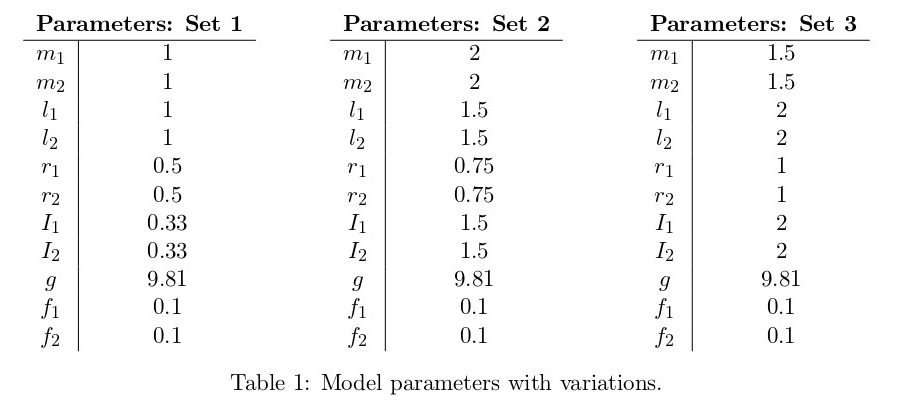
\includegraphics[width=0.7\linewidth]{parameters.png}
    \caption{model parameters with variations}
    \label{fig:enter-label}
\end{figure}
\section{Computation of the discretized dynamics function}
\begin{justify}
    {We developed this step by writing the function $discretizedDynamicFRA()$ that, as it say, implements the dynamics of the flexible robotic arm (FRA) in a discretized form. In order to define it, we followed the procedure outlined below: }
\end{justify}
\begin{itemize}
    {\item Firstly, we introduced and defined the Inertia matrix $M$, the Coriolis forces matrix $C$, the Gravity forces matrix $G$ and the Friction forces matrix $F$.
    \item Then, we proceeded by computing the first derivative of all the elements defined in the previous step.
    \item Lastly, we coded the actual dynamic in order to compute the state at the next istant of time (alias \( x_{t+1} \)) and we also coded the definition of the jacobians of the dynamic itself w.r.t. \(x\) and \(u\): \[\frac{\partial f}{\partial x}, \quad \frac{\partial f}{\partial u}\].} 
\end{itemize}
\section{Running the dynamic forward in time}
\begin{justify}
    {In order to be able to simulate the evolution of the dynamic forward in time given a certain initial state and a certain input curve, we defined the function  $runDynamicFunction$. This function requires as arguments:}
\end{justify}
\begin{itemize}
    {\item \textbf {$discretizedDynamicFunction$}: this must be a well defined function that takes as arguments the state and input values at time \(t\), and returns the state value at time \(t+1\) (alias \(\mathbf{x}_{t+1}\)) and all jacobians of the dynamics with respect to state and input (such it is for $discretizedDynamicFRA$), in the following order: \[\mathbf{x}_{t+1}, \quad \frac{\partial f}{\partial \mathbf{x}}, \quad \frac{\partial f}{\partial \mathbf{u}},\]
    \item {$uu$}: the input curve.
    \item {$xx_{0}$}: the fixed initial state.
    \item {$TT$}: number of time steps (each with duration \(dt\)), sufficient to evolve from \(t = 0\) to \(t = T\), where \([0, T]\) is the considered time horizon.}  
\end{itemize}
\begin{justify}
    {In a nutshell, we are initializing the state trajectory \(\mathbf{x}\) with the given initial state \(\mathbf{x}_{0}\) and then iterating a loop through $t = 0$ to $T-1$ relying on the given input \(\mathbf{u}\) and on the $discretizedDynamicFunction$ to generate the state at each time step.}
\end{justify}

\chapter{Task 1 - Optimal trajectory between two equilibria}
\section{Task description}
\begin{justify}
    {The first aim of task 1 is to compute two equilibria for our system and define a reference curve between the two. Then we have to proceed by computing the optimal transition to move from one equilibrium to another exploiting the Newton\textquotesingle s-like algorithm (in closed-loop version) for optimal control.}
\end{justify}
\section{Equilibria computation and definition of the reference curve between them}
\begin{justify}
    {For what concern the first part of this task, we define two equilibrium points thanks to the function implemented inside the equilibria.py file, $searchFRAInputGivenAnEquilibria$, that has as argument the scalar equilibrium value for $x_{0}$ (alias $-x_{1}$) and returns the scalar input value that generates the requested equilibrium point.
    \\Once the equilibrium points are defined we proceed by defining the reference curve between them. Firstly, we decide on the time instants in which the desired input-space curve will evolve, opting for $T = array([0, 5, 11, 16])$. Then we defined our desired state curve, thanks to the function $generateCurves(xxValues, uuValues, ttValues, curveTypeValues)$, as an exponential spline (generated in the function $exponentialSpline(t_1, t_2, v_1, v_2, dt)$), where the single spline's parameter has been tuned to minimize the variance of the curvature (normalized w.r.t its mean value) of the curve itself. After that, the input curve is generated by considering the angle of the first link of the FRA (at each time instant) and by searching the corresponding input value that leads to the equilibrium in which the first link is placed like that and the second link is pointing downwards (alias at the same angle but with opposite sign). \\All of that leds to a behaviour of the following type: from 0 to 5 seconds we have a constant section at the first equilibrium point, then from 5 to 11 seconds we have the evolving section, in which our curve reaches the second equilibrium point, lastly, from 11 to 16 seconds we continue with another constant section. We can conclude that our desired trajectory will vary inside a range that goes from -60 degrees to +60 degrees, for a total swing of 120 degrees. Before we proceed, let\textquotesingle s take a minute to analyze the function $generateCurves(xxValues, uuValues, ttValues, curveTypeValues)$. As said before, is used for the generation of curves for states. These curves are generated interpolating the given points at the given times. Each segment of the curve can be generated by using a sigmoid, a cubic spline or an exponential spline. This function takes as arguments:}
\end{justify}
\begin{itemize}
    \item $xxValues$ = ns x p sequence of states values to interpolate (where p is the numberOfPoints)
    \item $uuValues$ = ni x p sequence of inputs values to interpolate (if None, only the states curve is generated)
    \item $ttValues$ = 1 x p sequence of times values (ttValues[i] and ttValues[i+1] are the time instants of the i-th segment, with i from 0 to p-1)
    \item $curveTypeValues$ = 1 x (p-1) sequence of spline types to use for each segment
    (this value can also be passed as a scalar; in this case the same provided spline type is used for all the segments)
\end{itemize}
\begin{flushleft}
    Also, the function returns:
\end{flushleft}
\begin{itemize}
    \item $xx$ = ns x TT sequence of states values (where TT is the number of time steps and is computed as int(ttValues[-1]/dt))
    \item $uu$ = ni x TT sequence of inputs values
    \item $t$ = 1 x TT sequence of time values
\end{itemize}
\section{Optimal trajectory via Newton\textquotesingle s like algorithm}
\begin{justify}
    {Once that we complete the first step we can proceed by defining the cost matrices (that define the cost function) for the trajectory tracking optimization problem, this step is needed to represents how accurately we want to track a variable and allow us to apply the Newton\textquotesingle s method later on. We choose a matrix Q = diag[12, 12, 12, 12], used for the state variables, that we can describe as a diagonal matrix with 12 as both positions and velocities costs, and R = 0.001*eye(ni), used for the input variable, that we can describe as a diagonal matrix with 0.001 on the diagonal used for the input variable. Notice that R will be a one element matrix since we have just one input. After defining a maximum number of iteration for the newton\textquotesingle s method and a tolerance for it, we can now run the Newton\textquotesingle s method itself in order to minimize the cost function. In it we are using a regularized approach to avoid computing the Hessians of the dynamics.
    Let\textquotesingle s see now, specifically, the function that implements the Newton\textquotesingle s method and all the other functions that are involved within it:}
\end{justify}
\begin{itemize}
    \item $runNewtonMethodTrkTrj(xx_{des}, uu_{des}, maxIterations, \\ discretizedDynamicFuntion,tolerance, QQ, RR, QQT=None,\\ fixedStepsize=None)$ \\
    This function contain the overall newton\textquotesingle s like method in closed loop version for an optimal control trajectory generation problem. The arguments of this function are:
    \begin{itemize}
        \item $xx_{des}$ = a column vector state desired curve of dimension ns*TT where ns is the number of states of the system. We can describe its usage as: for t=0 we have the initial state $xx_0$, then we have the state curve for t from 1 up to T-2, then value for t=T-1 is considered as the state terminal value.
        \item $uu_{des}$ = a column vector input desired curve of dimension ni*TT where ni is the number of inputs of the system. We can describe its usage as: for t from 0 to T-2, we have the input curve;
        for t=T-1 we MUST have the input value that MUST be of equilibria for the system dynamic if considered within the terminal state value; it is also important that the state-input couple ad time t=0 is an equilibrium for the system dynamic.
        \item $maxIterations$ = maximum number of allowed iterations for the method to converge.
        \item $discretizedDynamicFunction$ =
        this function implements the discretized dynamics of the system that is being considered, requiring as arguments respectively the state and input values at time t, returning the state value at time t+1 and all the jacobians of the dynamic with respect to state and input in the following order: xxp, dfdx, dfdu.
        \item $tolerance$ = minimum value that the norm of the descent direction has to reach to consider the optimization as converged and completed.
        \item $QQ$ = ns*ns stage state cost matrix, if it is time invariant, or ns*ns*TT stage state cost tensor, if it is time variant.
        \item $RR$ = ni*ni stage input cost matrix (if time invariant) or ni*ni*TT stage input cost tensor (if time variant).
        \item $QQT$ = ns*ns terminal state cost matrix. Note that if None, the solution of the ARE (Algebric Riccati Equation) at t=T-1 is used for the terminal cost.
        \item $fixedStepsize$ = fixed stepsize to use for the optimization, if none option is present, the Armijo's rule is exploited to compute the stepsize.
        \item $generateNicePlots$ = flag to enable the generation of nice plots for the Armijo's rule (if True, the method generates the plots)
    \end{itemize}
    For what concern the elements that it returns, we have:
    \begin{itemize}
        \item $xx$ = column vector state of a feasible trajectory obtained through the optimization. It is coupled with uu in order to return a state-input trajectory.
        \item $uu$ = column vector input of a feasible trajectory obtained through the optimization. It is coupled with xx in order to return a state-input trajectory.
    \end{itemize}
    \item $solveCostateEquation(xx, uu, xx_{des}, uu_{des}, discretizedDynamicFuntion,\\ stageCostFunction, termCostFunction, TT)$ = implementation of the backwards-in-time solution of the costate equation of an Optimal Control Problem. The arguments of this function are:
    \begin{itemize}
        \item $xx$, $uu$, $xx_des$, $uu_des$, $discretizedDynamicFunction$ all previously defined.
        \item $stageCostFunction$ = this is the function that computes the cost associated with each stage of the process. In an optimal control problem, each time step or stage has a cost that depends on the current state and the control input. Thus, this function, represents the cost at each time step of the optimization process.
        \item $termCostFunction$ = Instead, this function computes the terminal cost, which is the cost associated with the final stage of the optimization problem. In optimal control problems, there is often a terminal cost that depends only on the final state of the system. Therefore, it takes the final state $xx_{des}$ as input and returns the terminal cost associated with that state.
        \item $TT$ = is the time horizon of our problem.
    \end{itemize}
    This function returns:
    \begin{itemize}
        \item $lmbda$ = the costate trajectory, alias the solution of the costate equation (lmbda) 
        \item $AA, BB$ = the jacobians of the dynamic w.r.t. x and w.r.t. u at x,u at each time step (respectively AA and BB)
        \item $QQdyn, SSdyn, RRdyn$ = the transposed hessians of the dynamic w.r.t. x and w.r.t. u at x,u at each time step (Qdyn as d2fdxdx, Sdyn as d2fdxdu, Rdyn as d2fdudu)
        \item $qq, rr$ = the transposed jacobians of the stage cost w.r.t. x and w.r.t. u at x,u at each time step (respectively q and r)
        \item $qqT$ = the transposed jacobian of the terminal cost w.r.t. x at the terminal state value (alias qT)
        \item $QQtilde$, $RRtilde$, $SStilde$ = the [transposed] hessians of the stage cost w.r.t. x and w.r.t. u at x,u at each time step (Qtilde as d2lldxdx, Stilde as d2lldxdu, Rtilde as d2lldudu)
        \item $grdJdu$ = the gradient of the cost function (expressed as only a function of the input) at $xx$,$uu$ at each time step (alias grdJdu) 
        \item $ll$ = the acutal cost associated to the given trajectory $xx$,$uu$ having $xx_des$, $uu_des$ as desired curves (alias l)
    \end{itemize}
    \item $solveAffineLQP(AA, BB, QQ, RR, SS, QQT, TT, xx_0, qq, rr, qqT)$\\
    Implementation of the solution of an affine linear quadratic optimal control problem solver.
    \item $solveLQP(AA, BB, QQ, RR, QQT, TT, xx0)$\\
    Implementation of the solution of a linear quadratic optimal control problem solver.
    \item $armijoStepSize(uu, xx, xx_{des}, uu_{des}, ll, direction, grdJdu, KK, sigma,\\ TT, discretizedDynamicFuntion, stageCostFunction, terminalCostFunction,\\ stepsizeInitialGuess = None)$\\
    Armijo's rule for step size selection, this is used to find an appropriate step size that ensures sufficient decrease in the cost function.The loop terminates when a satisfactory step size is found, or after a maximum number of iterations. If no satisfactory step size is found, the function selects the best step size from those tested. The arguments of our function are:
    \begin{itemize}
        \item $uu, xx, xx_{des}, uu_{des}, ll, grdJdu, KK, sigma, TT,\\ discretizedDynamicFuntion, stageCostFunction, terminalCostFunction$ all previously defined.
        \item $direction$ = a direction vector representing the direction in which to perturb the current control trajectory (uu) in order to minimize the cost.
        \item $stepsizeInitialGuess$ = an optional initial guess for the step size. If not provided, a default value of 1 is used.
    \end{itemize}
    The function returns:
    \begin{itemize}
        \item $stepsize$ = the selected step size based on Armijo's rule. This is the final step size that satisfies the Armijo condition for sufficient decrease in the cost function.
        \item $armijoStepsizes$ = a list of the stepsizes that were tested during the Armijo line search process.
        \item $armijoCosts$ = a list of the corresponding costs evaluated at each tested step size.
    \end{itemize}
    \item $solveARE(A, B, Q, R, S)$:\\
    Used to solve the Algebraic Riccati Equation (ARE), which is a key equation in optimal control theory, particularly in the Linear Quadratic Regulator (LQR) and other control problems. The arguments of this function are:
    \begin{itemize}
        \item $A$ = state transition matrix 
        \item $B$ = control input matrix
        \item $Q$ = state cost weight matrix in the quadratic cost function
        \item $R$ = control cost weight matrix in the quadratic cost function
        \item $S$ = additional matrix that is included in the augmented system. It is used to account for additional cross-coupling between state and control inputs. If S is provided and contains non-zero values, the system is augmented and solved accordingly.
    \end{itemize}
    The function returns the solution to the Algebraic Riccati Equation (ARE) or the augmented ARE, which is the optimal cost matrix P.
    \item $updateInputStateTrajectory(ns, ni, xx_0, uu_{old}, xx_{old}, stepsize, deltau,\\ KK, sigma, TT, discretizedDynamicFuntion):$\\
    This function updates the control inputs and state trajectory for a given system using a step size and perturbations to the control input. It handles both open-loop and closed-loop versions depending on the availability of feedback control parameters (K, sigma). Its arguments are:
    \begin{itemize}
        \item $ns, ni$ = number of states and inputs of the system 
        \item $xx0$ = initial state vector
        \item $xx_{old}$, $uu_{old}$ = previous state and control trajectory over time, which represents the state and control inputs at each time step.
        \item $stepsize$ = The step size used to scale the control perturbation
        \item $deltau$ = The perturbation (change) to the control inputs, typically a matrix of size (ni, T), which indicates how the control inputs will be adjusted.
        \item $KK, sigma, TT, discretizedDynamicFunction$ = all previously defined.
    \end{itemize}
    The function returns:
    \begin{itemize}
        \item $uu_{new}$, $xx_{new}$ = the updated control and state trajectory over time.
    \end{itemize}
    In addition, we define the class $TrjTrkOCPData$ containing the following methods:\\ $setEndingTime$, $getElapsedTime$, $getOptimalTrajectory$,\\ $getOptimalCostGradient$, $getOptimalTrajectoryErrorsAtFinalTime$.
\begin{flushleft}
    Now we can look at the required plot obtained from all this work.
\end{flushleft}
\begin{figure}[ht]
    % Immagine a sinistra
    \begin{minipage}[t]{0.48\textwidth}
        \centering
        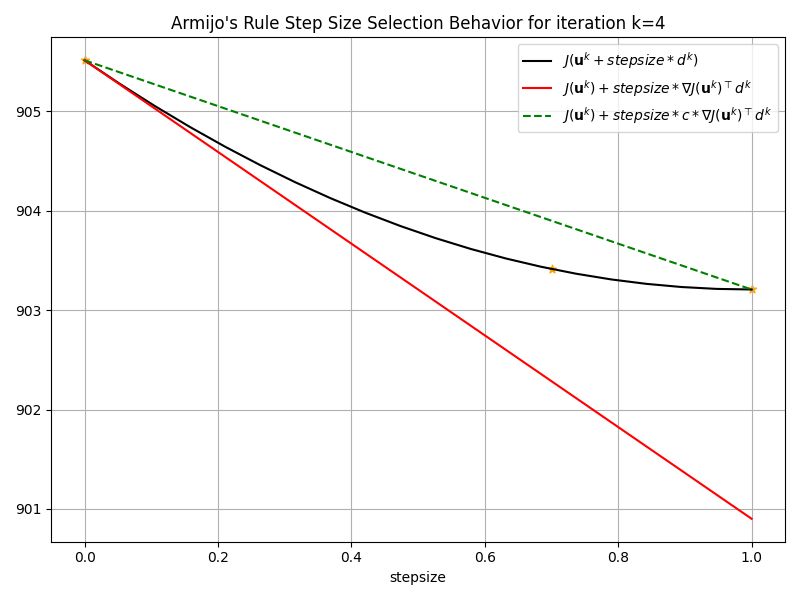
\includegraphics[width=\textwidth]{Armijo's_Rule_K=3_T1.png}
        \caption{Armijo's rule for k = 4}
        \label{fig:sinistra}
    \end{minipage}
    \hfill
    % Immagine a destra
    \begin{minipage}[t]{0.48\textwidth}
        \centering
        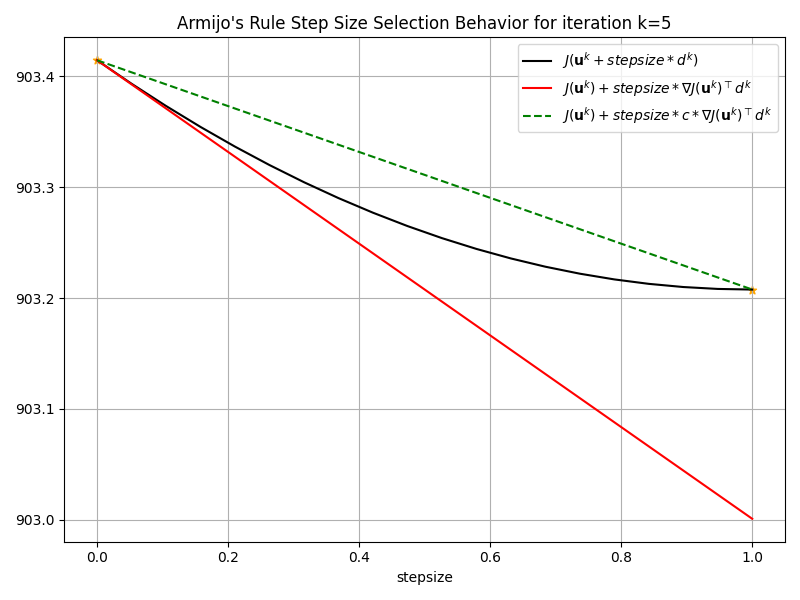
\includegraphics[width=\textwidth]{Armijo's_Rule_K =4_T1.png}
        \caption{Armijo's rule for k = 5}
        \label{fig:destra}
    \end{minipage}
\end{figure}
\begin{figure}[ht]
    % Immagine a sinistra
    \begin{minipage}[t]{0.48\textwidth}
        \centering
        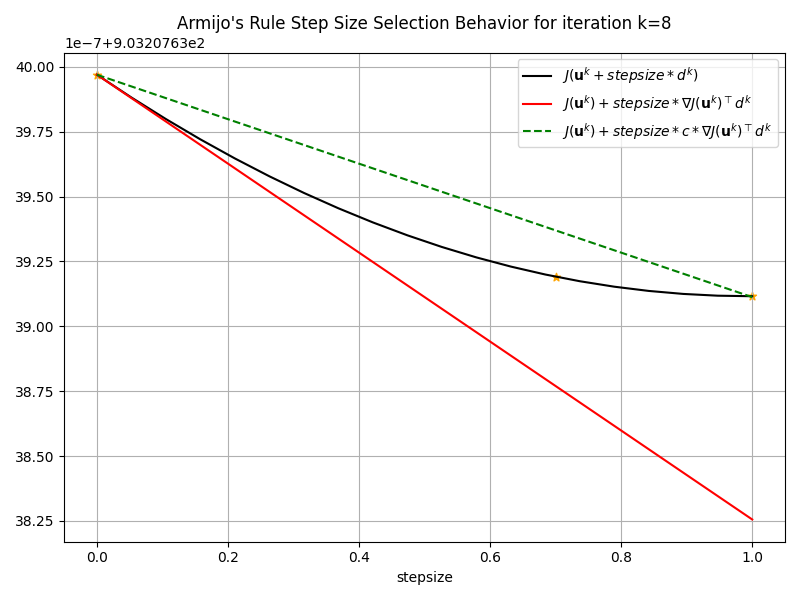
\includegraphics[width=\textwidth]{Armijo's_Rule_T1_k=8.png}
        \caption{Armijo's rule for k = 8}
        \label{fig:sinistra}
    \end{minipage}
    \hfill
    % Immagine a destra
    \begin{minipage}[t]{0.48\textwidth}
        \centering
        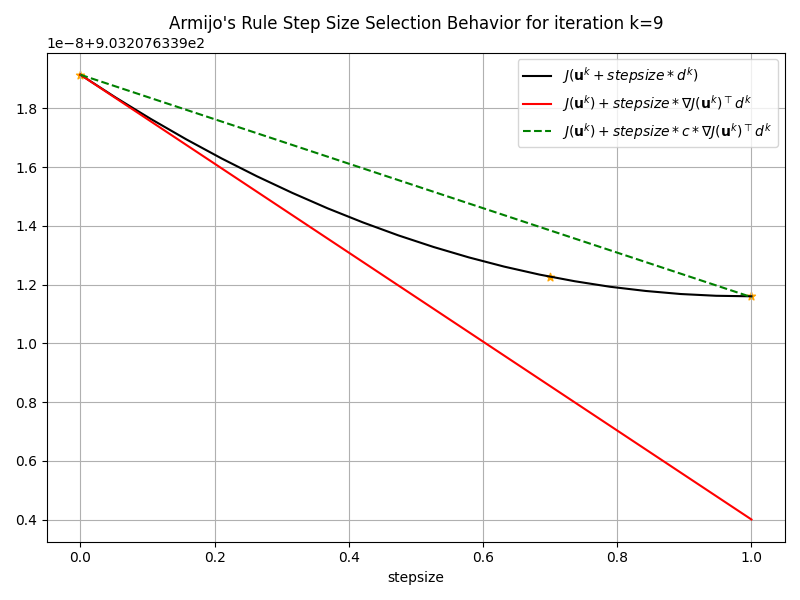
\includegraphics[width=\textwidth]{Armijo's_Rule_T1_k=9.png}
        \caption{Armijo's rule for k = 9}
        \label{fig:destra}
    \end{minipage}
\end{figure}

\begin{figure}[H]
    \centering
    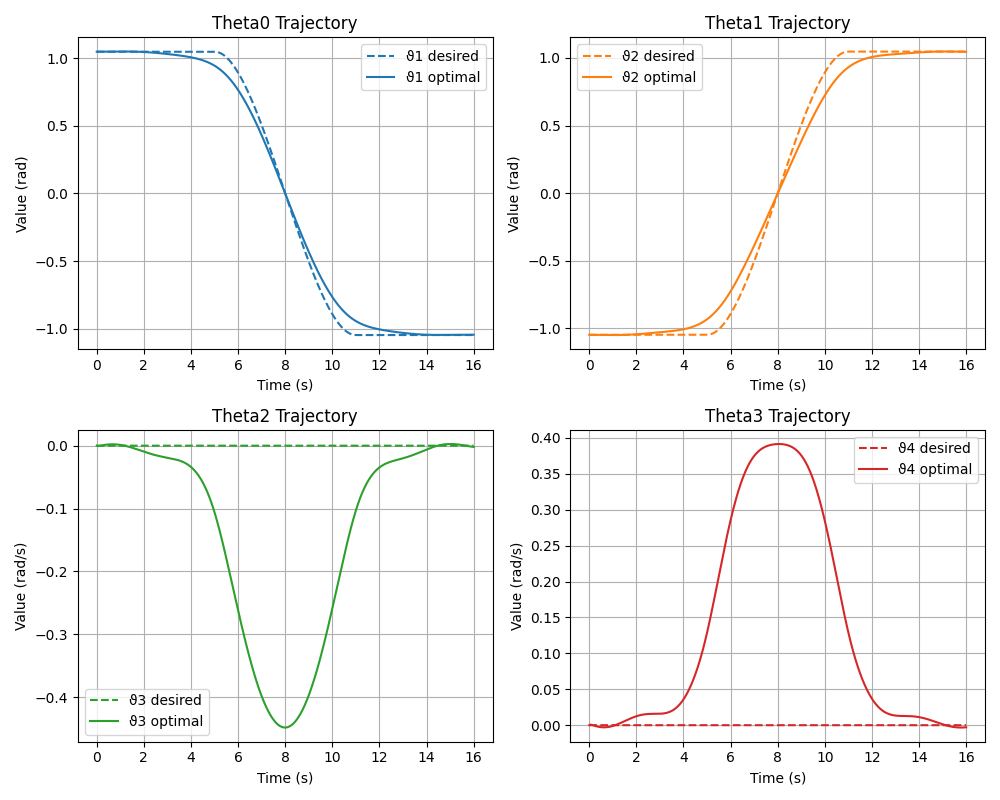
\includegraphics[width=0.8\textwidth]{States_Trajectories_T1.png}
    \caption{Desired and optimal trajectories}
    \label{fig:enter-label}
\end{figure}
\begin{figure}[H]
    \centering
    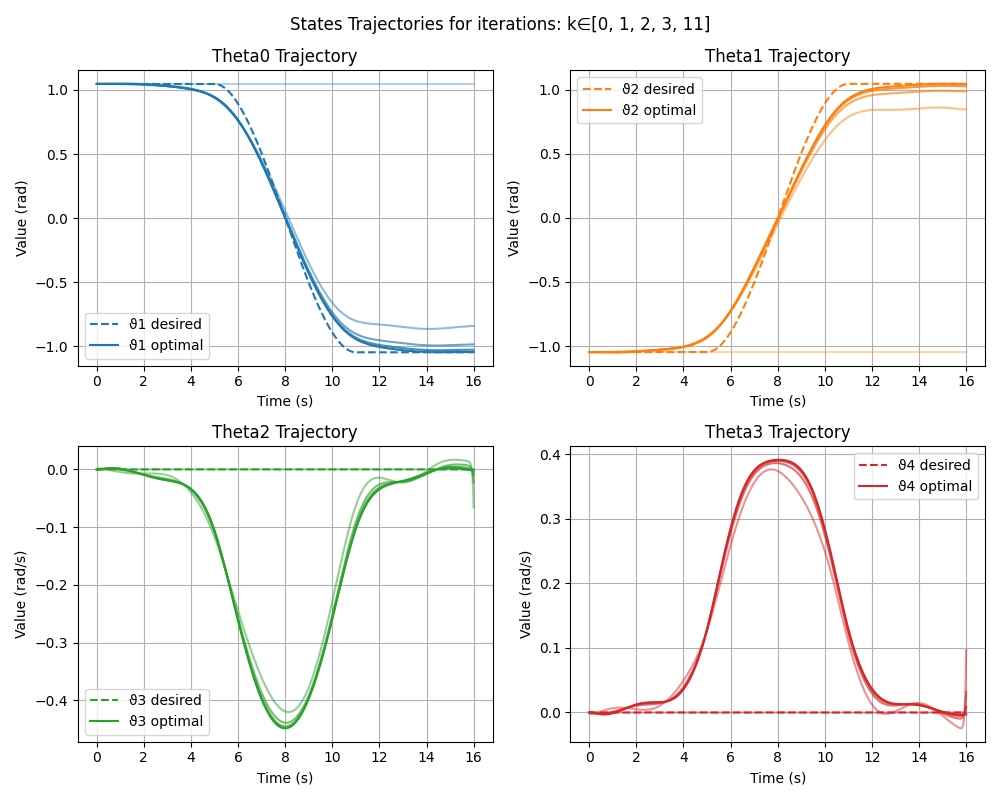
\includegraphics[width=0.8\textwidth]{States_Trajectories_for_iterations_T1.png}
    \caption{Intermediate iteration to obtain the optimal trajectories}
    \label{fig:enter-label}
\end{figure}
\begin{figure}[ht]
    % Immagine a sinistra
    \begin{minipage}[t]{0.48\textwidth}
        \centering
        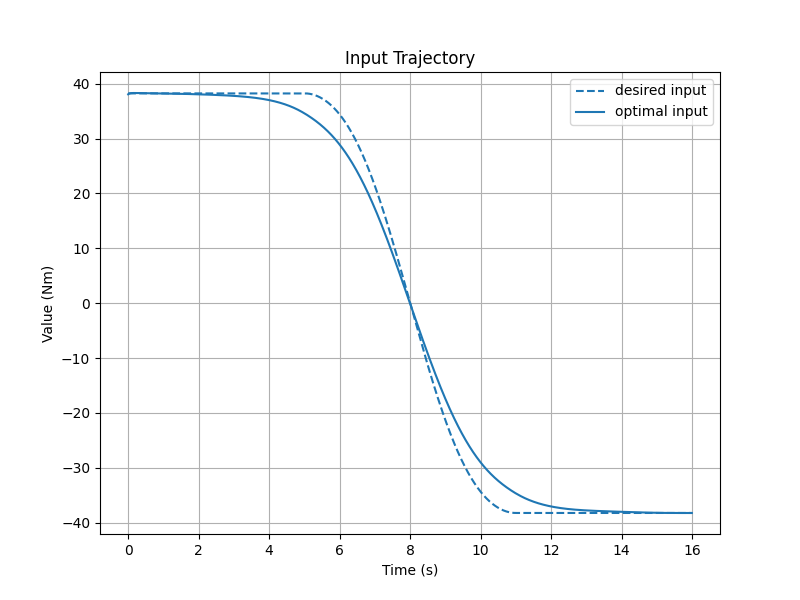
\includegraphics[width=\textwidth]{Input_Trajectory_T1.png}
        \caption{Desired and optimal input trajectories}
        \label{fig:sinistra}
    \end{minipage}
    \hfill
    % Immagine a destra
    \begin{minipage}[t]{0.48\textwidth}
        \centering
        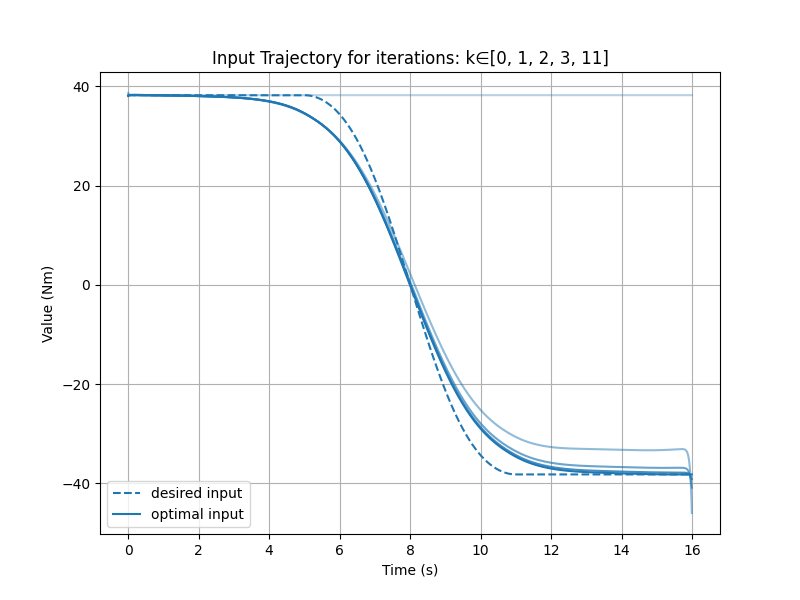
\includegraphics[width=\textwidth]{Input_Trajectory_for_iterations_T1.png}
        \caption{Intermediate iteration to obtain the optimal input trajectory}
        \label{fig:destra}
    \end{minipage}
\end{figure}

\begin{figure}[ht]
    % Immagine a sinistra
    \begin{minipage}[t]{0.48\textwidth}
        \centering
        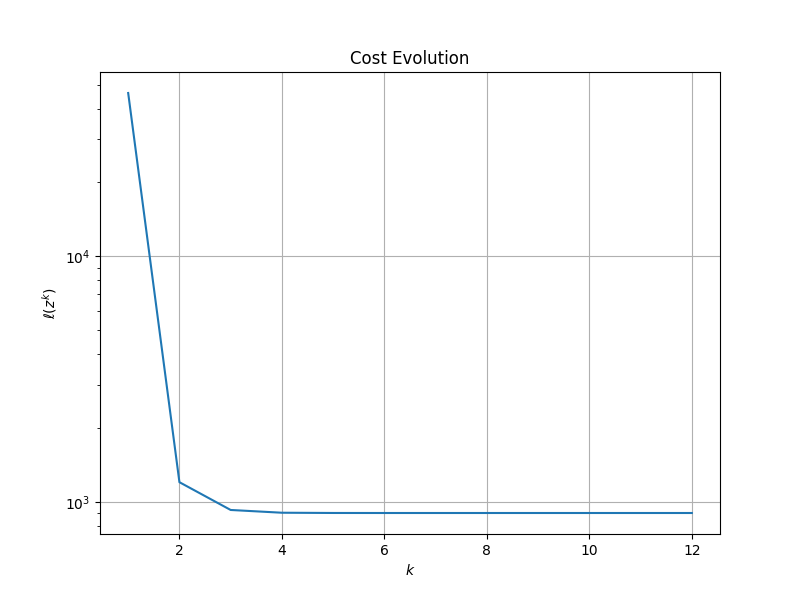
\includegraphics[width=\textwidth]{Cost_Evolution_T1.png}
        \caption{Obtained decrease for the cost function evolution}
        \label{fig:sinistra}
    \end{minipage}
    \hfill
    % Immagine a destra
    \begin{minipage}[t]{0.48\textwidth}
        \centering
        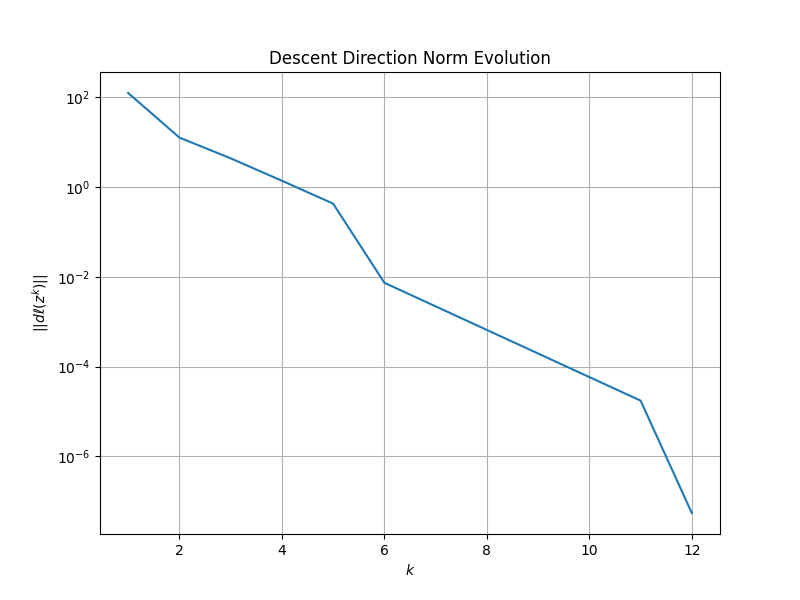
\includegraphics[width=\textwidth]{Descent_Direction_T1.png}
        \caption{Obtained decrease for the norm of descent direction}
        \label{fig:destra}
    \end{minipage}
\end{figure}
\end{itemize}
\newpage
\section{Conclusions}

\begin{justify}
    {The results demonstrate the effectiveness of using a Newton-like algorithm in a closed-loop framework to compute the optimal control trajectories for transitioning between two equilibria of our system. All the plots are a demonstration of what just said, let's focus on them individually. The descent direction norm evolution plot confirms the rapid convergence of the optimization algorithm within 10 iterations, indicating efficient optimization. The cost evolution plot further proves this efficiency, as the cost function quickly stabilizes after the initial iterations. The intermediate trajectory plots for the system variables $(theta0, theta1, theta2, theta3)$ show that the desired and optimal trajectories align closely, ensuring smooth transitions between the equilibria while respecting the constraints. Additionally, the input trajectories demonstrate precise control inputs that facilitate the desired state transition without excessive energy usage. Finally, the Armijo plots across iterations validate the step size selection strategy, ensuring that the optimization progresses steadily. These results highlight the algorithm's capability to achieve optimal state transitions with high accuracy, stability, and computational efficiency. While working with the Newton\textquotesingle s method we face the importance of the cost matrices tuning, in particular for what concern R since it allow us to balance the trade-off between minimizing control effort and achieving the desired state trajectories, ensuring smooth trajectories.}
\end{justify}

\chapter{Task 2 - Newton\textquotesingle s method on smooth trajectory}
\section{Task description}
\begin{justify}
    {The goal we have to accomplish for this second task of our project is to generate a desired (smooth) state input curve and perform the trajectory generation task (Task 1) on this new desired curve. In Task 1, the goal was to achieve a transition between two equilibrium points, without the need of following a trajectory perfectly. For this reason, we used a step-like fitting, but made smoother through an exponential function. In addition, we assigned the same weight to the costs for position and velocity. This allowed Newton's method to develop an optimal solution by considering position and velocity with equal importance, avoiding favoring one component at the expense of the other.
    In Task 2, however, the goal is different, in particular we have to define and follow a more complex trajectory in position. To achieve this, we introduce one main change from Task 1.
    \begin{itemize}
        \item Cost balancing: we proceed by assigning significantly higher costs to positions than to velocities. This allowed us to focus the optimization on good trajectory tracking in position, achieving the main objective of Task 2.
    \end{itemize}
    In summary, recalibrating costs is the key steps to achieve the desired outcome in Task 2, in contrast to the focus on simply linking equilibria in Task 1.}
\end{justify}
\section{Equilibria computation}
\begin{justify}
    {We define the reference trajectory, with the same procedure we adopted for Task 1, so we need to define  the time instants in which the desired input-space curve should evolve, opting for $T = array([0, 5, 9, 13, 17, 21, 26])$. Then we define our desired input-state curve, thanks to the function $generateCurves(xxValues, uuValues, ttValues, curveTypeValues)$ as a series of exponential-spline-junctions between a set of equilibrium points, that is generated by considering the angle of the first link of the FRA (at each time instant) and by searching the corresponding input value that leads to the equilibrium in which the second link is pointing downwards (alias at the same angle but with opposite sign). This lead us to a behaviour of the following type: from 0 to 5 we start from the first equilibrium point and we have a constant section, then from 4 to 21 we have multiple evolving sections through the equilibrium points, lastly, from 21 to 26 we end with another constant section. We can conclude that our desired trajectory will vary inside a range that goes from -30 degrees to +90 degrees, for a total maximum swing of 120 degrees.}
\end{justify}
\section{Newton\textquotesingle s method on smooth curve}
\begin{justify}
    {We can proceed now, as we did for Task 1, therefore, once that we complete the first step we can proceed by defining the cost matrices, and in particular a diagonal matrix Q = diag([16, 16, 6, 6]) to describe the state variables and a diagonal matrix R = 0.001*eye(ni) used for the input variable, we can notice that RR will be a one element matrix since we have just one input. As said previously, we introduce these matrices to define the cost function, for the trajectory tracking optimization problem, in fact this step is needed to represent how accurately we want to track a variable and allow us to apply the Newton\textquotesingle s method after the definition of a maximum number of iterations and a tolerance. The application of this method enable us to minimize the cost function. This minimization is of main importance for the computation of the descent direction, in which we can avoid to compute the Hessian of the dynamics by solving the costate equations and solving an affine linear quadratic problem. Inside paragraph 2.3 we described all the functions we had to develop to compute the Newton\textquotesingle s method and other procedures mentioned above, since nothing changes from the previous task except for what already mentioned, we won't report and describe all the functions again. However we will obviously obtain different plots, therefore, I will report them here.}
\end{justify}

\clearpage

\begin{figure}[ht]
    % Immagine a sinistra
    \begin{minipage}[t]{0.48\textwidth}
        \centering
        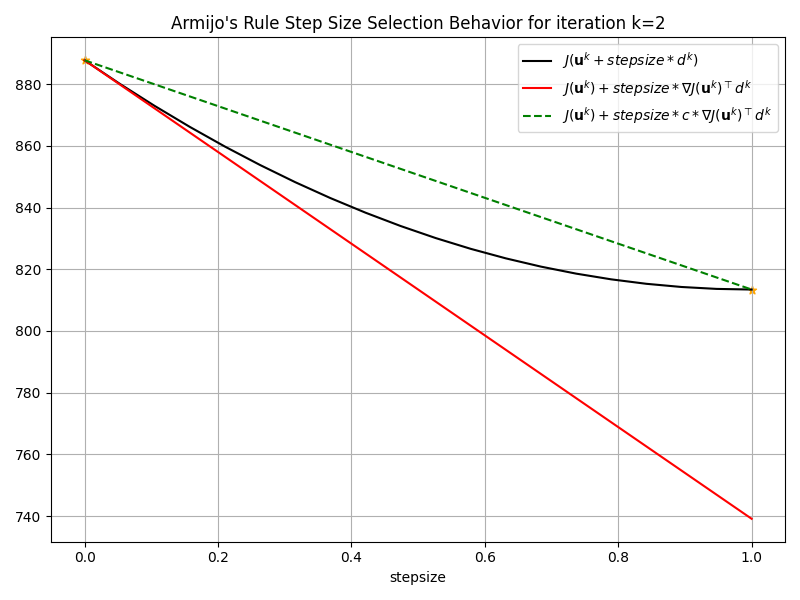
\includegraphics[width=\textwidth]{Armijo's_Rule_T2_k=2.png}
        \caption{Armijo's rule for k = 2}
        \label{fig:sinistra}
    \end{minipage}
    \hfill
    % Immagine a destra
    \begin{minipage}[t]{0.48\textwidth}
        \centering
        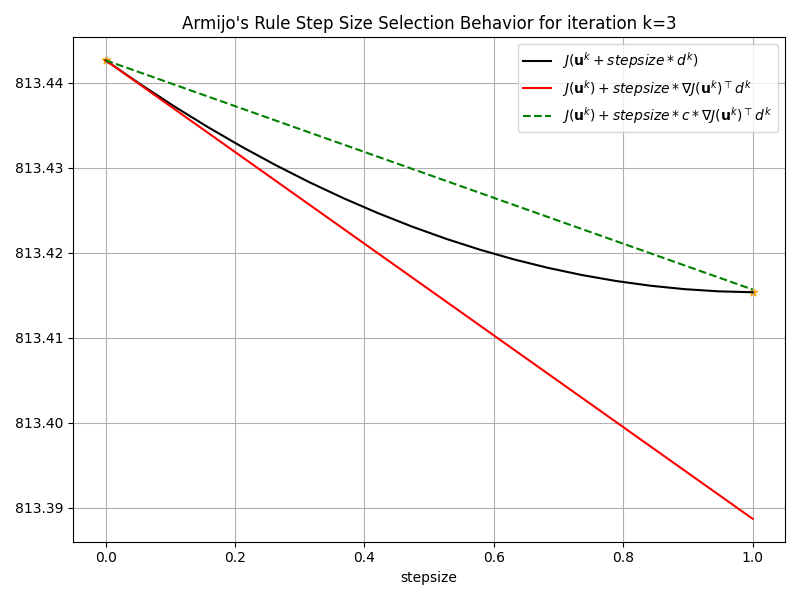
\includegraphics[width=\textwidth]{Armijo's_Rule_T2_k=3.png}
        \caption{Armijo's rule for k = 3}
        \label{fig:destra}
    \end{minipage}
\end{figure}
\begin{figure}[H]
    \centering
    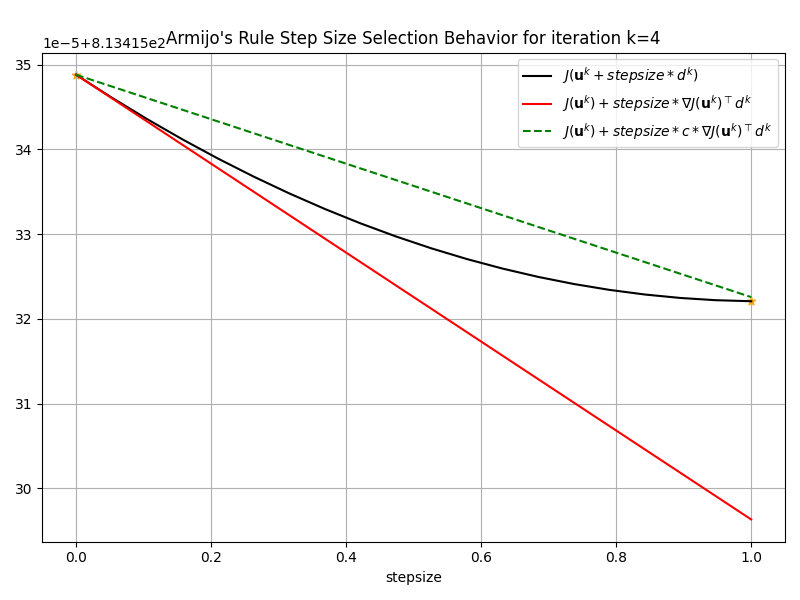
\includegraphics[width=0.48\textwidth]{Armijo's_Rule_T2_k=4.png}
    \caption{Armijo's rule for k = 4}
    \label{fig:enter-label}
\end{figure}
\begin{figure}[H]
    \centering
    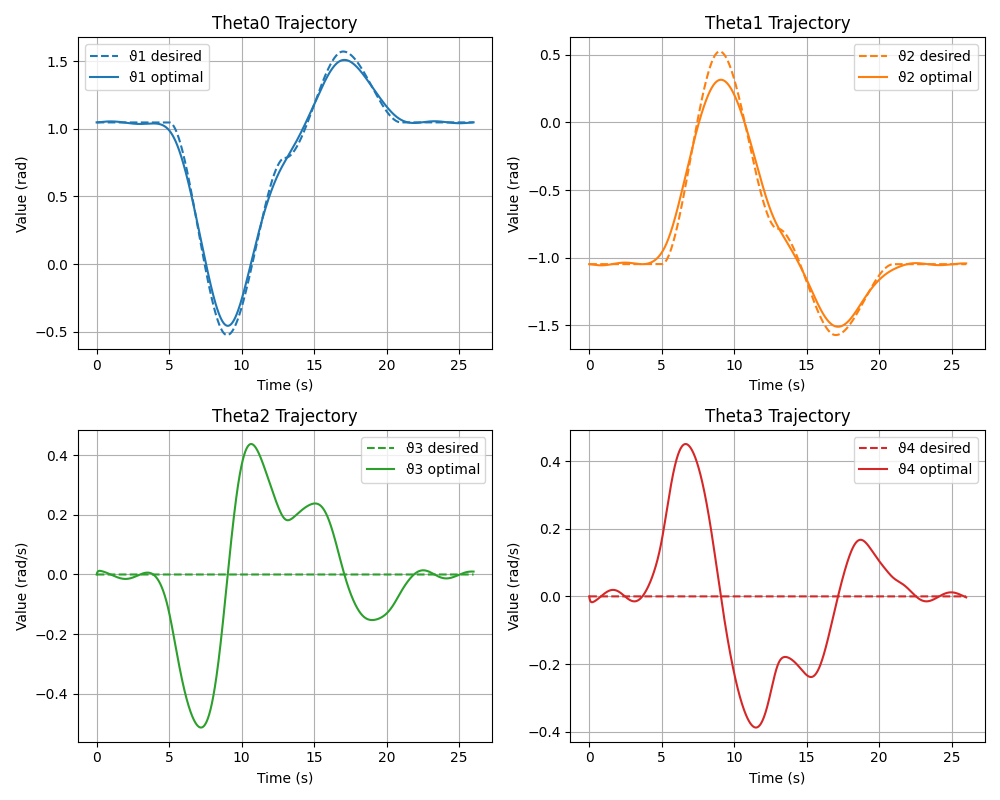
\includegraphics[width=0.8\textwidth]{States_Trajectories_T2.png}
    \caption{Desired and optimal trajectories}
    \label{fig:enter-label}
\end{figure}
\begin{figure}[H]
    \centering
    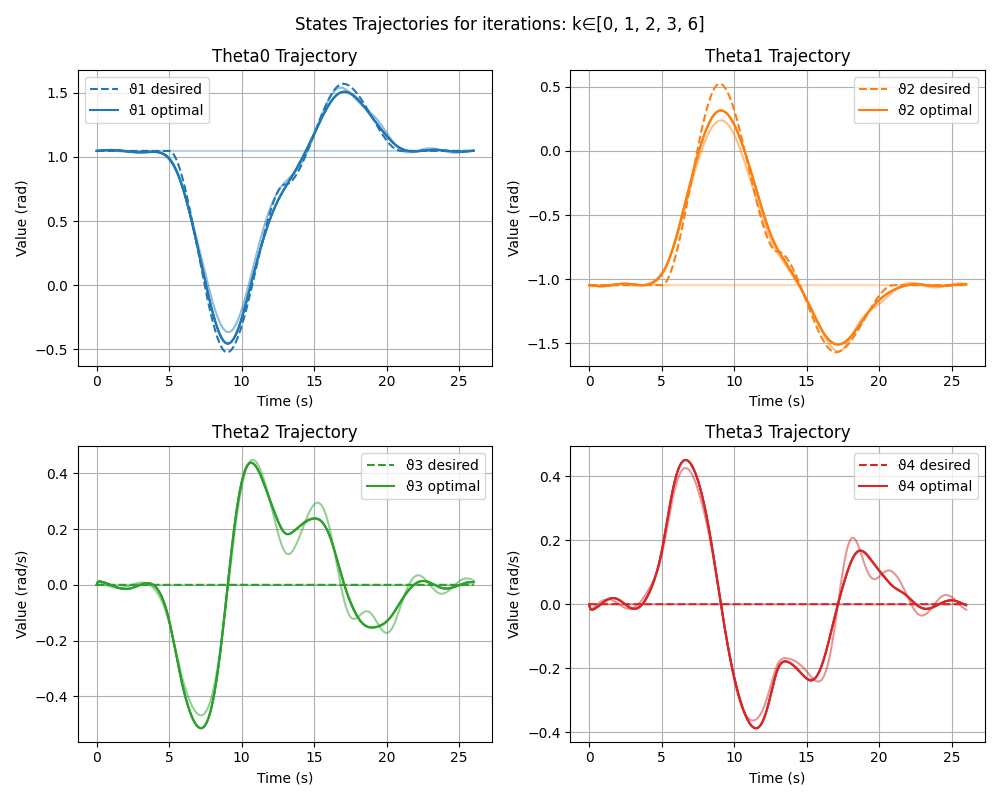
\includegraphics[width=0.8\textwidth]{States_Trajectories_for_iterations_T2.png}
    \caption{Intermediate iterations to obtains the optimal trajectories}
    \label{fig:enter-label}
\end{figure}
\begin{figure}[ht]
    % Immagine a sinistra
    \begin{minipage}[t]{0.48\textwidth}
        \centering
        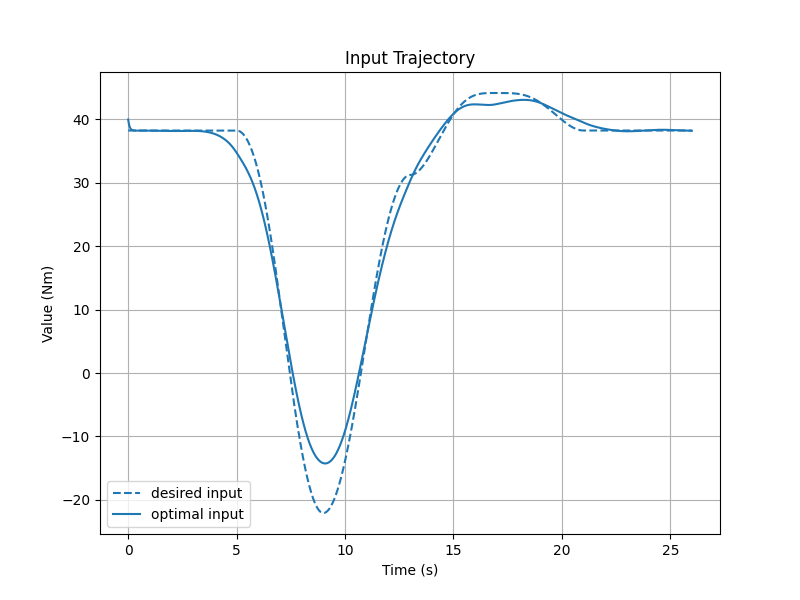
\includegraphics[width=\textwidth]{Input_Trajectory_T2.png}
        \caption{Desired ad optimal input trajectories}
        \label{fig:sinistra}
    \end{minipage}
    \hfill
    % Immagine a destra
    \begin{minipage}[t]{0.48\textwidth}
        \centering
        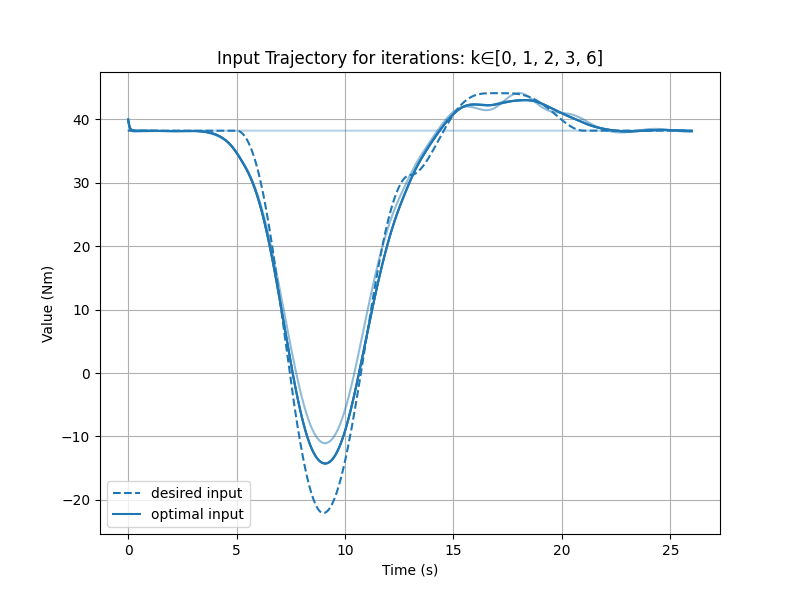
\includegraphics[width=\textwidth]{Input_Trajectory_for_iterations_T2.png}
        \caption{Intermediate iterations to obtains the optimal input trajectories}
        \label{fig:destra}
    \end{minipage}
\end{figure}

\begin{figure}[ht]
    % Immagine a sinistra
    \begin{minipage}[t]{0.48\textwidth}
        \centering
        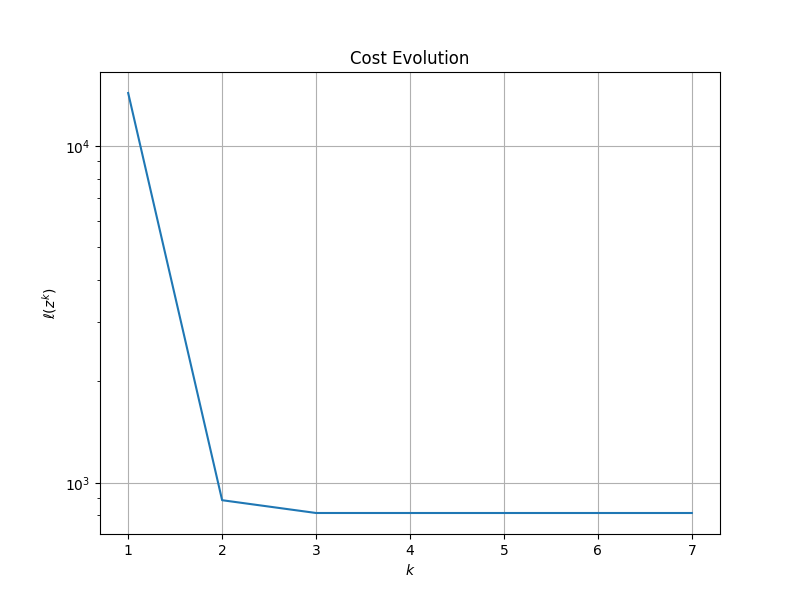
\includegraphics[width=\textwidth]{Cost_Evolution_T2.png}
        \caption{Obtained decrease for the cost function evolution}
        \label{fig:sinistra}
    \end{minipage}
    \hfill
    % Immagine a destra
    \begin{minipage}[t]{0.48\textwidth}
        \centering
        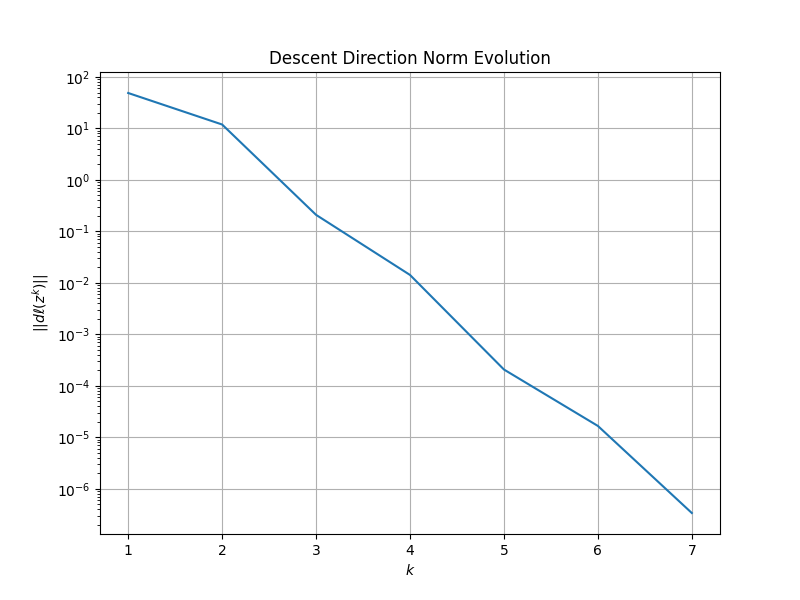
\includegraphics[width=\textwidth]{Descent_Direction_T2.png}
        \caption{Obtained decrease for the norm of descent direction}
        \label{fig:destra}
    \end{minipage}
\end{figure}
\clearpage
\section{Conclusions}
\begin{justify}
    {The results showcase the effectiveness of employing a Newton\textquotesingle s like algorithm within a closed-loop framework to compute optimal control trajectories for transitioning between two equilibria of the system. Each plot provides clear evidence supporting this conclusion. The descent direction norm evolution plot highlights the rapid convergence of the algorithm, achieving optimization within just 6 iterations, demonstrating its robustness and efficiency. Similarly, the cost evolution plot confirms this efficiency, as the cost function stabilizes quickly after the initial iterations. The intermediate trajectory plots for the system variables $(theta0, theta1, theta2, theta3)$ reveal a close alignment between the desired and optimal trajectories, ensuring smooth transitions between equilibria while adhering to constraints. The input trajectories further validate the precision of the control inputs, enabling the desired state transition with minimal energy expenditure. Moreover, the Armijo plots across iterations confirm the effectiveness of the step size selection strategy, facilitating steady and consistent optimization progress. These findings underline the algorithm\textquotesingle s ability to achieve accurate, stable, and computationally efficient state transitions. Finally, the results emphasize the critical role of tuning the cost matrices, particularly $R$, to balance the trade-off between minimizing control effort and achieving smooth, desired state trajectories.}
\end{justify}

\chapter{Task 3 - Trajectory tracking via LQR}
\section{Task description}
\begin{justify}
    {In this third task what was asked was to linearize the robot dynamics about the generated trajectory $(x^{\text{gen}}, u^{\text{gen}})$ computed in Task 2, exploit the LQR algorithm to define the optimal feedback controller to track this reference trajectory and in particular, to solve the LQ Problem:}
\end{justify}
\begin{center}
    {$&\min_{\Delta x_1, \dots, \Delta x_T, \Delta u_0, \dots, \Delta u_{T-1}} \quad \sum_{t=0}^{T-1} \Delta x_t^\top Q^{\text{reg}} \Delta x_t + \Delta u_t^\top R^{\text{reg}} \Delta u_t + \Delta x_T^\top Q_T^{\text{reg}} \Delta x_T \\
    &\text{subject to} \quad \Delta x_{t+1} = A_t^{\text{gen}} \Delta x_t + B_t^{\text{gen}} \Delta u_t, \quad t = 0, \dots, T-1 \\
    &\quad \quad \quad \quad \quad x_0 = 0$}
\end{center}
\begin{justify}
    {where $A_t^{\text{gen}}, B_t^{\text{gen}}$ represent the linearization of the (nonlinear) system about the optimal trajectory. Considering the fact that the cost matrices of the regulator are our degree-of-freedom.
    In summary, our goal was to design a linear quadratic regulator (LQR) able to follow the smooth optional trajectory generated in the previous task.}
\end{justify}

\section{Description of the implemented solution}
\begin{justify}
    {We start to develop this task by linearizing the system dynamics computed in task 0, about the smooth optimal trajectory that we computed in task 2 through the functions $computeLocalLinearization$ contained in our dynamics file. It is possible to notice that we import the trajectory thanks to the $loadDataFromFIle()$ function, that avoid us the burden to recompute it for every task. Once obtained the matrix $A_{lin}$, $B_{lin}$ from the linearization we compute the gain $K$ as the solution of the LQP (linear quadratic optimization problem) given by the function $solveLQP$. In order to implement this function we use as $QQT$, therefore as terminal cost matrix, the ARE (Algebraic Riccati Equation) solution implemented in the function $solveARE$ and as Q and R the matrices defined in task 2. Concluded these steps we use the obtained $K$ to design the desired LQR (Linear Quadratic Regulator) defined in the function $runLQRController$. At this point, we test it with different noise levels, in particular we choose $xx0noiseLevels = [0.0, 0.2, 0.4]$ that will be used by the function $generateInitialStateNoise$, to see how it reacts to perturbations of the initial state while asked to follow the optimal trajectory. Let\textquotesingle s now analyze, in detail, all the function mentioned.}
\end{justify}
\begin{itemize}
    \item $computeLocalLinearization(xx_traj, uu_traj)$ = given a feasible state-input trajectory of states and inputs, this function computes the local linearization of the dynamics around that trajectory. It takes as arguments:
    \begin{itemize}
        \item $xx_{traj}$ = $ns*TT$ column vector state trajectory
        \item $uu_{traj}$ = $ni*TT$ column vector input trajectory
    \end{itemize}
    While it returns:
    \begin{itemize}
        \item $AA$ = $ns*ns*TT$ tensor of jacobians of the dynamics w.r.t. the state at each time instant
        \item $BB$ = $ns*ni*TT$ tensor of jacobians of the dynamics w.r.t. the input at each time instant
    \end{itemize}
    \item $solveLQP$ = this function solves a time-varying linear quadratic optimal control problem. It computes the optimal control and state trajectory for a discrete-time linear system with time-varying dynamics and quadratic cost function. This involves solving the backward Riccati Equation to obtain the cost matrices and gain matrices, followed by a forward simulation to calculate the optimal state and control trajectories. The algorithm is well-suited for trajectory tracking and optimal control of linearized systems. This because, it ensures efficient computation of control laws while minimizing a trade-off between control effort and state trajectory deviation. Its arguments are:
    \begin{itemize}
        \item $AA$, $BB$, $QQ$, $RR$, $QQT$, $TT$, $xx_{0}$ = all previously defined 
    \end{itemize}
    Instead, it returns:
    \begin{itemize}
        \item KK = array of optimal feedback gain matrices for every time step
        \item PP = array of cost matrices computed using the Riccati Equation
        \item $xx_{out}$ = array of the optimal state trajectory over time
        \item $uu_{out}$ =  array of the optimal control inputs over time 
    \end{itemize}
    \item $solveARE(A, B, Q, R, S):$\\ Used to solve the Algebraic Riccati Equation (ARE), which is a key equation in optimal control theory, particularly in the Linear Quadratic Regulator (LQR) and other control problems. The arguments of this function are:
    \begin{itemize}
        \item $A$ = state transition matrix 
        \item $B$ = control input matrix
        \item $Q$ = state cost weighting matrix in the quadratic cost function
        \item $R$ = control cost weighting matrix in the quadratic cost function
        \item $S$ =additional matrix that is included in the augmented system. It is used to account for additional cross-coupling between state and control inputs. If S is provided and contains non-zero values, the system is augmented and solved accordingly.
    \end{itemize}
    The function returns the solution to the Algebraic Riccati Equation (ARE) or the augmented ARE, which is the optimal cost matrix P.
    \item $runLQRController(xx_{traj}, uu_{traj}, KK, discretizedDynamicFunction,\\ xx0Noise = None, includeMeasureNoises = False)$ = this function run the LQR controller, using the given feedback gain KK, on the given trajectory. The arguments of this function are: 
    \begin{itemize}
        \item $xx_{traj}, uu_{traj}$ = the state and input reference trajectory
        \item $KK$ = the feedback gain matrix related to the LQR 
        \item = $discretizedDynamicFunction$ = a function that represents the discretized dynamic of the system
        \item $xx0noise$ = this is a noise to be eventually added to the initial stare
        \item $includeMeasureNoises$ = a boolean flag that indicates if the measure noises should be included in the simulation. In case, noises are added to the state trajectory at each time instant, where for each state the noise is generated by taking samples from a N(0,1) normal distribution scaled by a percentage of the maximum value assumed by the state itself along the trajectory.
    \end{itemize}
    This function returns:
    \begin{itemize}
        \item $xx_{track}, uu_{track}$ = the state and input trajectory, respectively tracked and applied by the LQR controller.
    \end{itemize}
    \item $generateInitialStateNoise(xx, noiseStdPercentage, gainK = 2,\\ randomNumberGenerator = None)$ = This function takes care of the generation of a noise to be added to the initial state of the system. That noise in generated (for each single state) by taking samples from a N(0,1) normal distribution scaled (in its standard deviation by the percentage of the standard deviation of the state itself). Its arguments are:
    \begin{itemize}
        \item xx = this is the state trajectory matrix where each row represents a different state variable over time. The function computes the standard deviation of each state variable (row-wise) to determine the noise scale.
        \item $noiseStdPercentage$ = a percentage (expressed as a fraction) that scales the noise standard deviation relative to the standard deviation of the state variables. If set to None or <= 0, the function will return a zero vector.
        \item $gainK$ = a multiplicative gain applied to further scale the noise standard deviation. Default is 2
        \item $randomNumberGenerator$ = A random number generator instance for producing reproducible noise. If not provided, a default generator seeded with 2828 is used.
    \end{itemize}
    It returns:
    \begin{itemize}
        \item noise = a 1D array of random Gaussian noise with the same size as the number of state variables (ns). The noise is scaled based on the computed standard deviations of the state variables and the user-specified parameters (noiseStdPercentage and gainK).
    \end{itemize}
\end{itemize}
\section{Results}
\begin{flushleft}
    Let\textquotesingle s see the plot that we obtained from the procedure that we just explained.
\end{flushleft}

\begin{figure}[H]
    \centering
    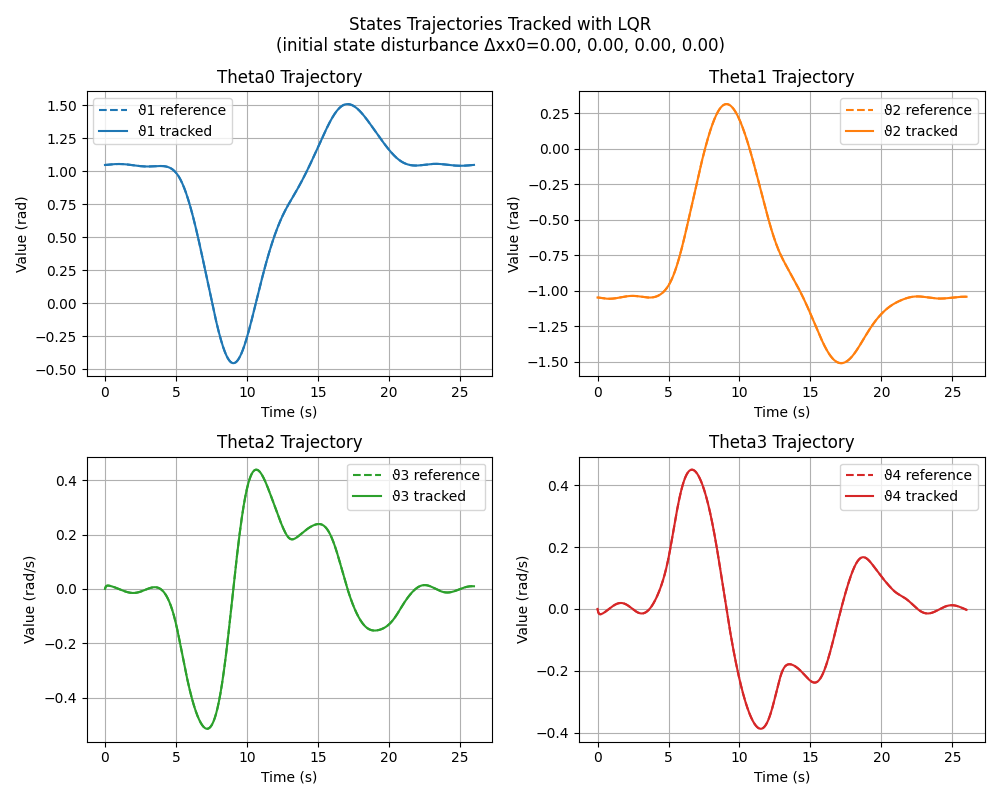
\includegraphics[width=0.8\textwidth]{States_Trajectories_Tracked_with_LQR_T3.png}
    \caption{States trajectories tracked with LQR and no disturbance}
    \label{fig:enter-label}
\end{figure}
\begin{figure}[H]
    \centering
    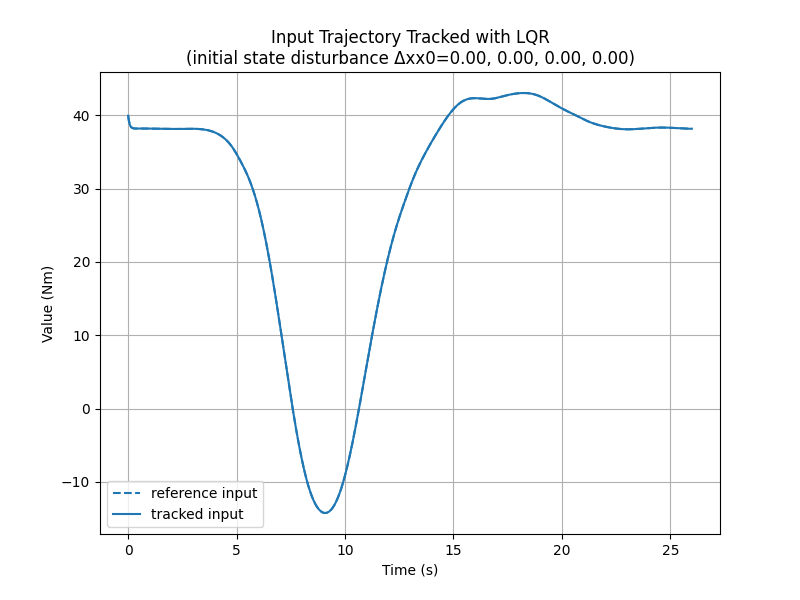
\includegraphics[width=0.8\textwidth]{Input_Trajectory_Tracked_with_LQR_T3.png}
    \caption{Input trajectory tracked with LQR and no disturbance}
    \label{fig:enter-label}
\end{figure}
\begin{figure}[H]
    \centering
    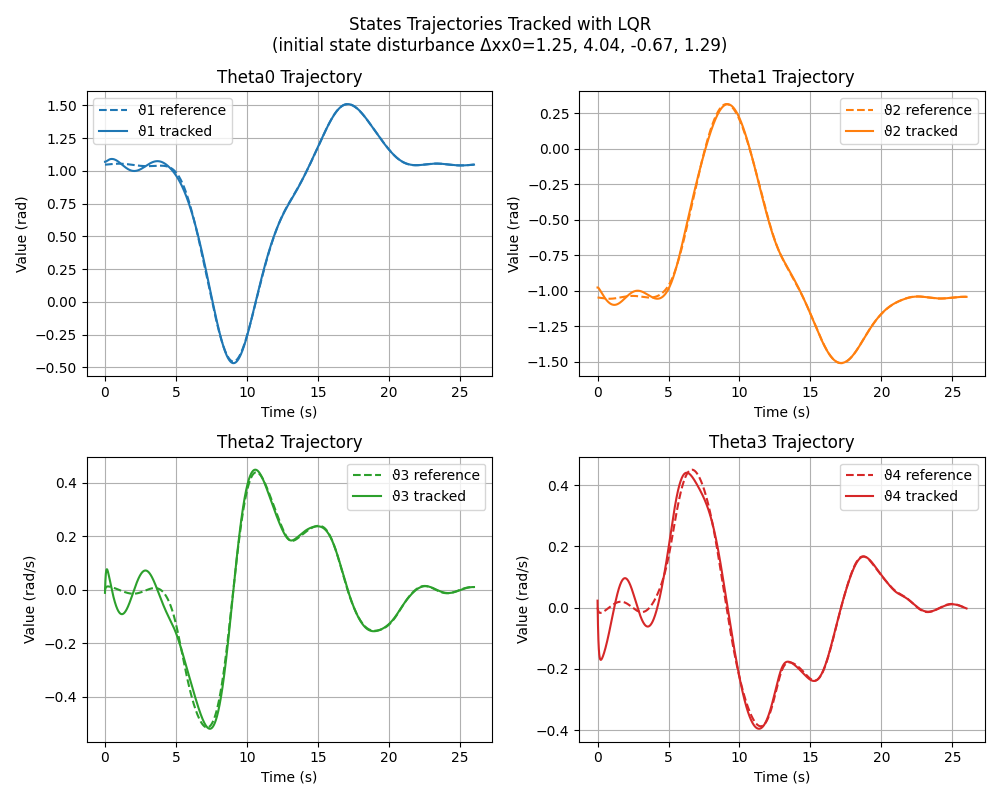
\includegraphics[width=0.9\textwidth]{States_Trajectories_Tracked_with_LQR_dist1_T3.png}
    \caption{States trajectories tracked with LQR and smaller disturbance}
    \label{fig:enter-label}
\end{figure}
\begin{figure}[H]
    \centering
    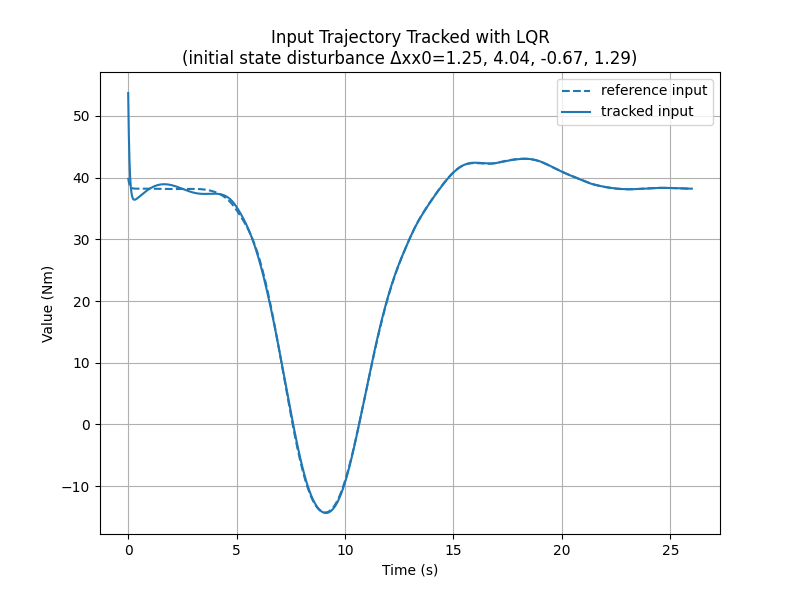
\includegraphics[width=0.9\textwidth]{Input_Trajectory_Tracked_with_LQR_dist1(I)_T3.png}
    \caption{Input trajectories tracked with LQR and smaller disturbance}
    \label{fig:enter-label}
\end{figure}
\begin{figure}[H]
    \centering
    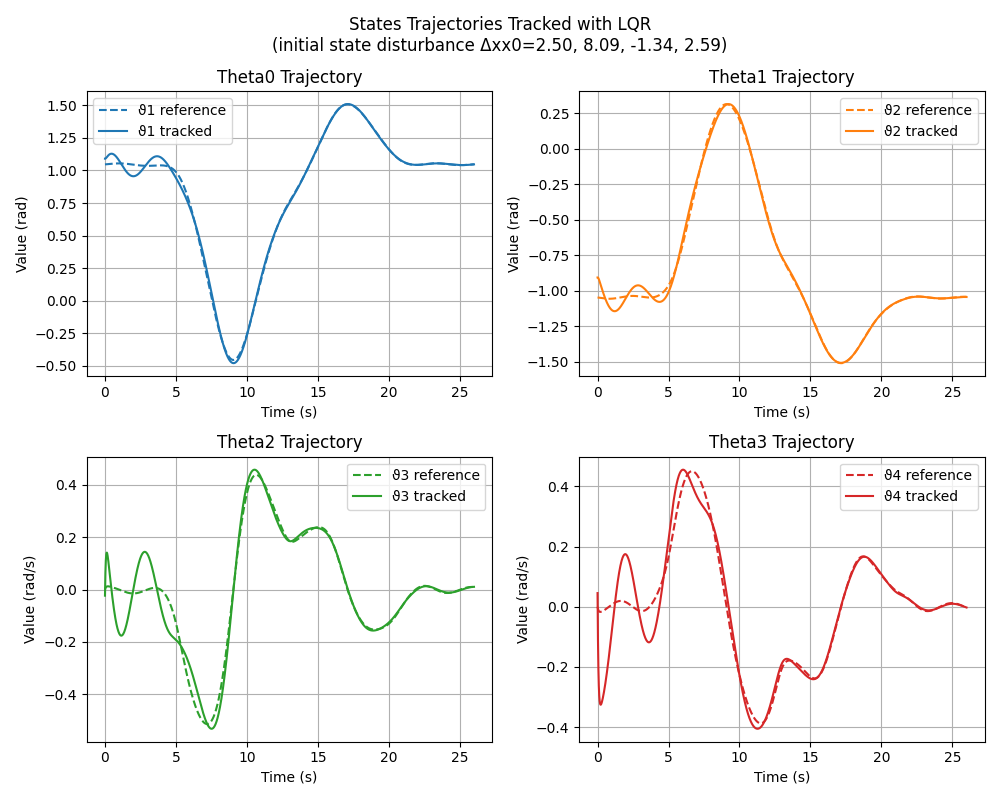
\includegraphics[width=0.9\textwidth]{States_Trajectories_Tracked_with_LQR_dist2_T3.png}
    \caption{States trajectories tracked with LQR and bigger disturbance}
    \label{fig:enter-label}
\end{figure}
\begin{figure}[H]
    \centering
    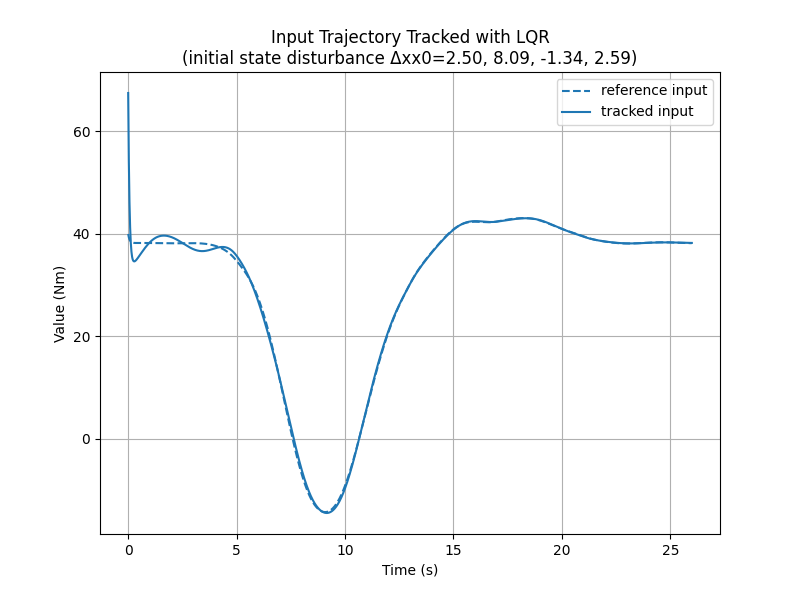
\includegraphics[width=0.9\textwidth]{Traj_tracked_dist2(I)_T3.png}
    \caption{Input trajectories tracked with LQR and bigger disturbance}
    \label{fig:enter-label}
\end{figure}

\begin{figure}[H]
    \centering
    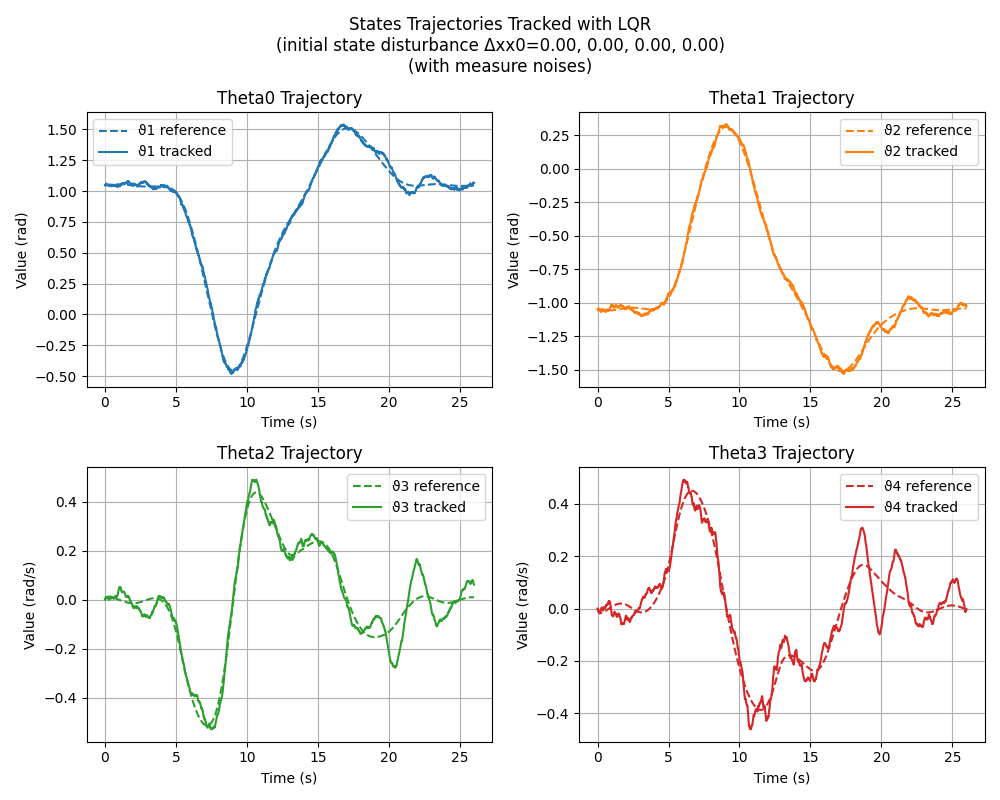
\includegraphics[width=0.85\textwidth]{LQR_mn_T3.png}
    \caption{States trajectories tracked with LQR and no disturbance, but with measure noise}
    \label{fig:enter-label}
\end{figure}
\begin{figure}[H]
    \centering
    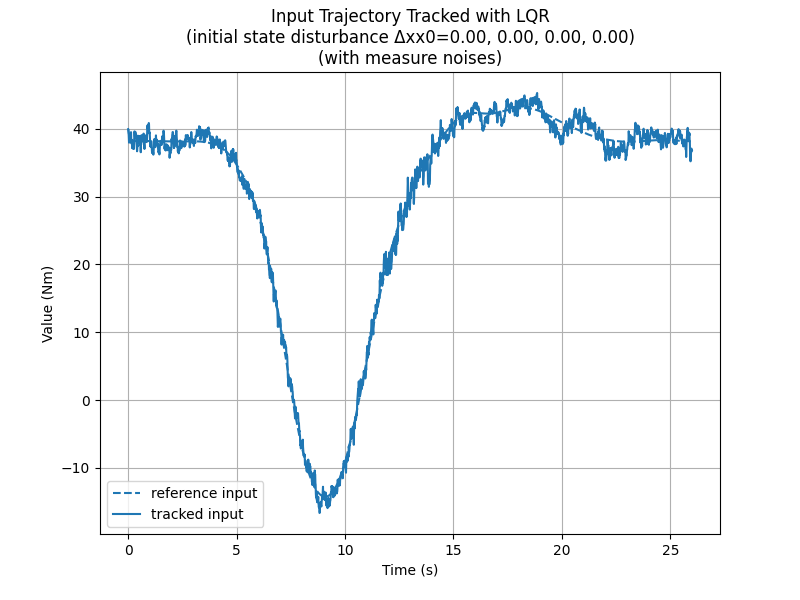
\includegraphics[width=0.85\textwidth]{Input_Trajectory_Tracked_with_LQR_mn_T3.png}
    \caption{Input trajectories tracked with LQR, no disturbance, but with measure noise}
    \label{fig:enter-label}
\end{figure}

\clearpage

\section{Conclusions}
\begin{justify}
    {Based on the results obtained from the implementation of the LQR controller, we can conclude that the designed feedback control law effectively tracks the reference trajectory generated in Task 2. The state and input trajectories shown in the plots illustrate the system's ability to follow the optimal path with minimal deviation. Furthermore, testing the controller under different noise levels demonstrates its robustness, as it successfully mitigates disturbances and maintains trajectory tracking performance. Higher noise levels introduce some deviations, as expected, but the control strategy ensures stability and convergence. Overall, the LQR-based approach provides a reliable and efficient solution for trajectory tracking in this robotic system, validating the theoretical framework and implementation.}
\end{justify}

\chapter{Task 4 - Trajectory tracking via MPC}
\section{Task description}
\begin{justify}
    {In this task we are asked to linearize the robot dynamics about the trajectory ($x_{gen},u_{gen}$) computed in Task 2, exploiting an MPC algorithm to track this reference trajectory.}
\end{justify}
\section{Description of the solution implemented}
\begin{justify}
    {The procedure we will follow is really similar to what we did to achieve our goal in task 3. In fact we begin this task by linearizing the system dynamics obtained in Task 0 around the smooth optimal trajectory generated in Task 2. This is done using the computeLocalLinearization function from our dynamics file. Notably, we retrieve the trajectory using the loadDataFromFile() function, which eliminates the need to recompute it for each task, simplifying the process. Once obtained AAlin e BBlin from the linearization, we define the prediction time horizon for the MPC, $MPC_{TT}$ and the cost matrices $Q=diag([16.0,16.0,6.0,6.0])$ and $R=0.0001*eye(ni)$. Once developed the MPC controller through the function $runMPController$, we proceed choosing with which noise levels perturbate our system in order to study how it reacts to disturbances while asked to follow the optimal trajectory. Aside from this, we also try to analyze our system under measure noises and additional constraints (e.i. input saturation). Let\textquotesingle s see now the new functions needed in this task to achieve our goal.}
\end{justify}
\begin{itemize}
    \item $runMPCController(xx_traj, uu_traj, AA, BB, QQ, RR, MPC_TT\\, discretizedDynamicFunction, xx0Disturbance = None,\\ generateMeasureNoises = False, useCVXSolver = True,\\ considerAdditionalConstraints = True)$ = this is the function that run the MPC controller on the given trajectory. it takes as arguments:
    \begin{itemize}
        \item $xx_{traj}$, $uu_{traj}$ = the state and input reference trajectories
        \item $AA$, $BB$ = matrix A and B of the linearized dynamics around the reference trajectory
        \item $QQ$, $RR$, $QQT$ = cost matrices that are supposed to be time invariant
        \item $MPC_TT$ = prediction time horizon for the MPC.
        \item $discretizedDynamicFunction$ = previously descripted
        \item $xx0Disturbance$ = a disturbance to be eventually added to the initial state
        \item $generateMeasureNoises$ = a boolean flag that indicates if already-set-up additional constraints should be considered. In case, the cvxpy library is used (instead of the analytic solver) to solve the LQ problems involved in the MPC action (in order to make it possible to take into account the additional constraints).
    \end{itemize}
    Our function returns:
    \begin{itemize}
        \item $xx_{traj}$, $uu_{traj}$ = the state and input respectively tracked and applied by the MPC controller
    \end{itemize}
    \item $cvxpyProblemSetup(ns, ni, QQ, RR, QQT, MPC_TT, considerAdditionalConstraints)$ = this function sets up the CVXPY problem for the MPC controller (if needed). Its arguments are:
    \begin{itemize}
        \item ns, ni = number of states and inputs
        \item QQ, RR = States and input cost matrices (supposed to be time invariant)
        \item $MPC_{TT}$ = already defined
        \item $considerAdditionalConstraints$ =  A boolean flag that indicates if already-set-up additional constraints should be considered.
    \end{itemize}
    The function returns:
    \begin{itemize}
        \item problem = the set-up CVXPY problem
        \item $xx_traj$, $uu_traj$ = The state and input CVXPY Variables (that correspond to the prediction that the MPC will compute at each instant of time)
        \item $xx_traj$, $uu_traj$ = The CVXPY Parameters related to the reference trajectory (that the MPC aims to track)
        \item $xx0_{real}$: The initial state CVXPY Parameter (that correspond to the actual real value of the state at current istant of time, beginning of the prediction horizon)
        \item AA, BB = The list of CVXPY Parameters related to the local linearization matrices (on the prediction horizon)
    \end{itemize}
    \item  $cvxpyProblemSolver(problem, xx_real, uu_real, xx0_real, AA, BB, xx_traj, uu_traj, xx0_real_val, AAval, BBval, xx_traj_val, uu_traj_val)$ = this function update CVXPY parameters and solve the problem. It takes as arguments:
    \begin{itemize}
        \item $problem, xx_{real}, uu_{real}, xx0_{real}, AA, BB,xx_{traj}, uu_{traj}$ = all previously defined.
        \item $xx0_{real_val}, AAval, BBval, xx_{traj_val}, uu_{traj_val}$ = correspond to the previously defined elements but thought for validation.
    \end{itemize}
    the function returns:
    \begin{itemize}
        \item $optimal_xx, optimal_uu$ = the optimized state and input trajectories.
        \item status = a flag indicating whether the solver successfully found a solution 
        \item cost = the objective function value at the optimal solution
        \item $validating_results$ = performance metrics or validation results using the test trajectory.
    \end{itemize}
\end{itemize}
\section{Results}
\begin{flushleft}
    Now we can look at the plot we obtained from the procedure just described. In particular for what concern the last four plots we analyze a possible solution we achieved by considering an hypothetic additional measure noise.
\end{flushleft}

\clearpage

\begin{figure}[H]
    \centering
    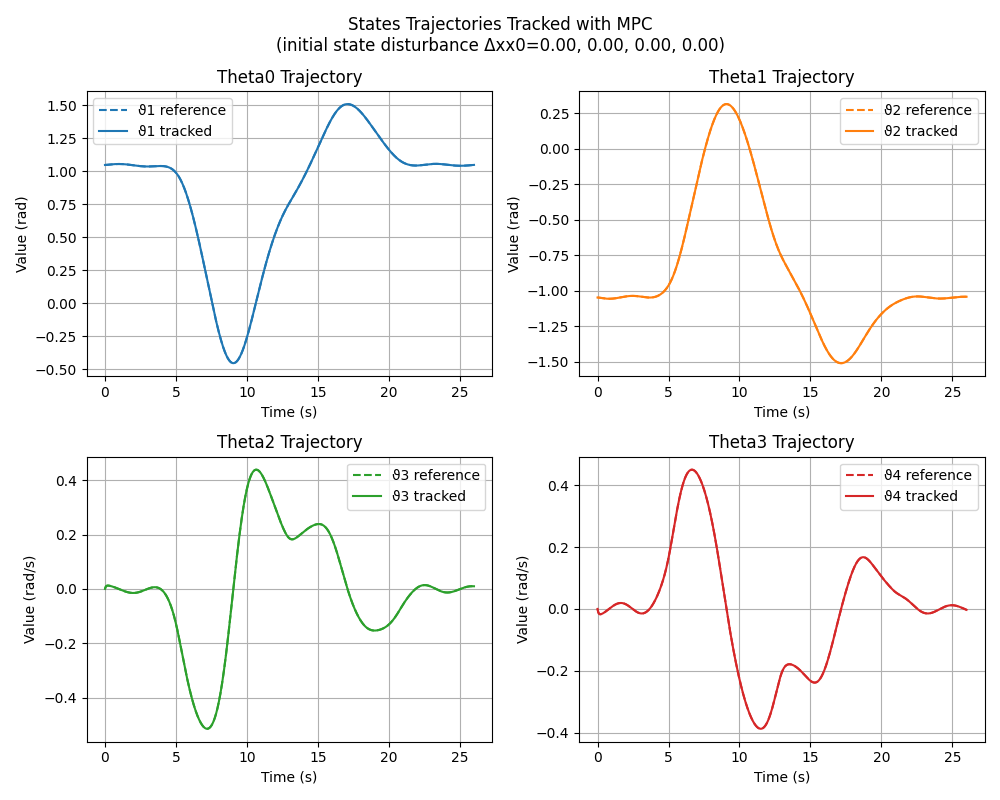
\includegraphics[width=0.9\textwidth]{State_traj_MPC_T4.png}
    \caption{States trajectories tracked with MPC and no disturbance}
    \label{fig:enter-label}
\end{figure}
\begin{figure}[H]
    \centering
    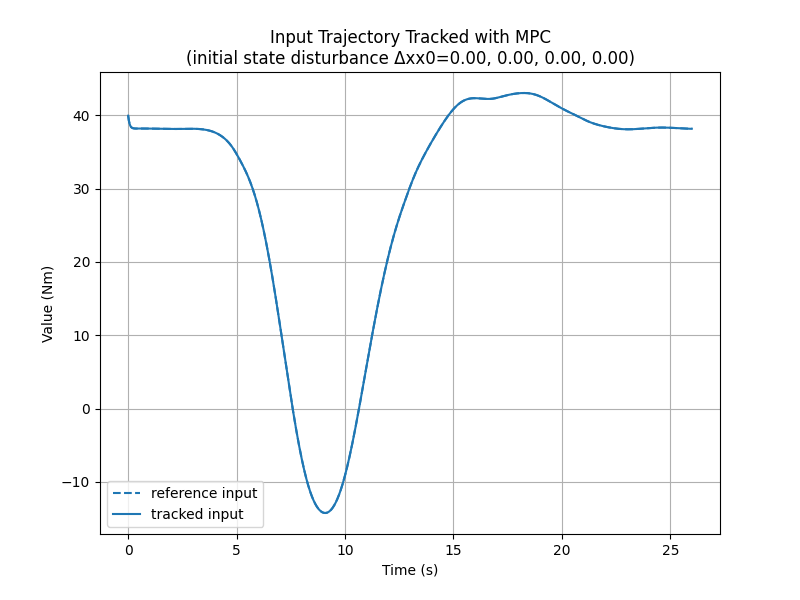
\includegraphics[width=0.9\textwidth]{Input_traj_MPC_T4.png}
    \caption{Input trajectories tracked with MPC and no disturbance}
    \label{fig:enter-label}
\end{figure}
\begin{figure}[H]
    \centering
    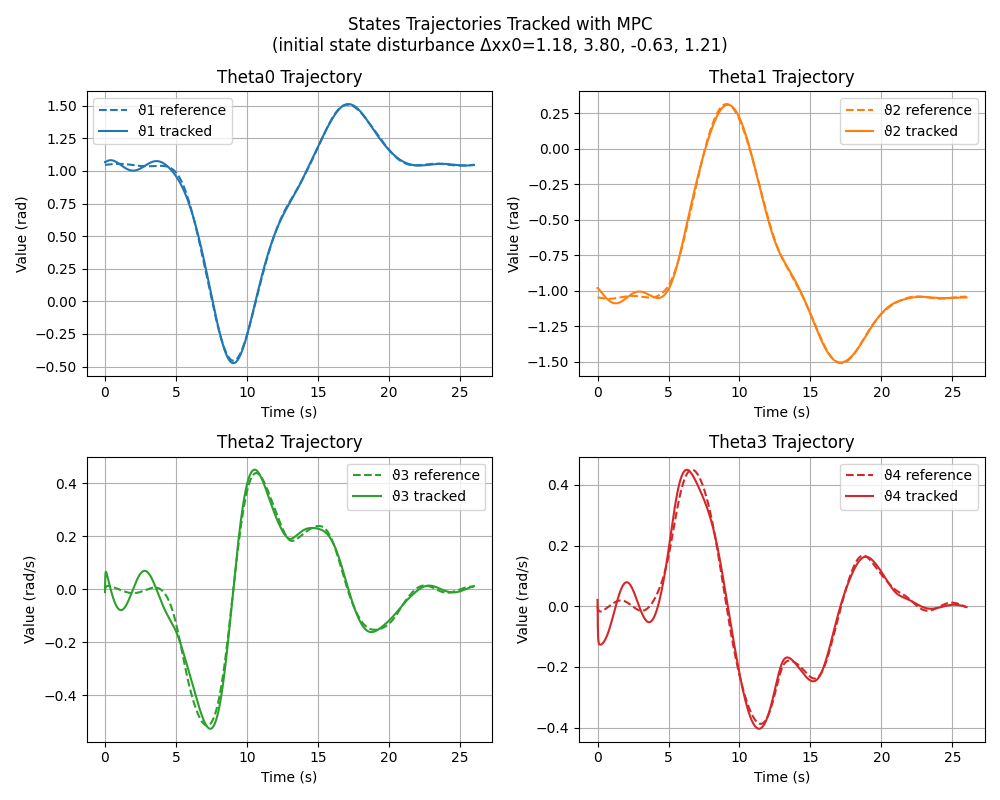
\includegraphics[width=0.9\textwidth]{State_traj_MPC_dist1_T4.png}
    \caption{States trajectories tracked with MPC and smaller disturbance}
    \label{fig:enter-label}
\end{figure}
\begin{figure}[H]
    \centering
    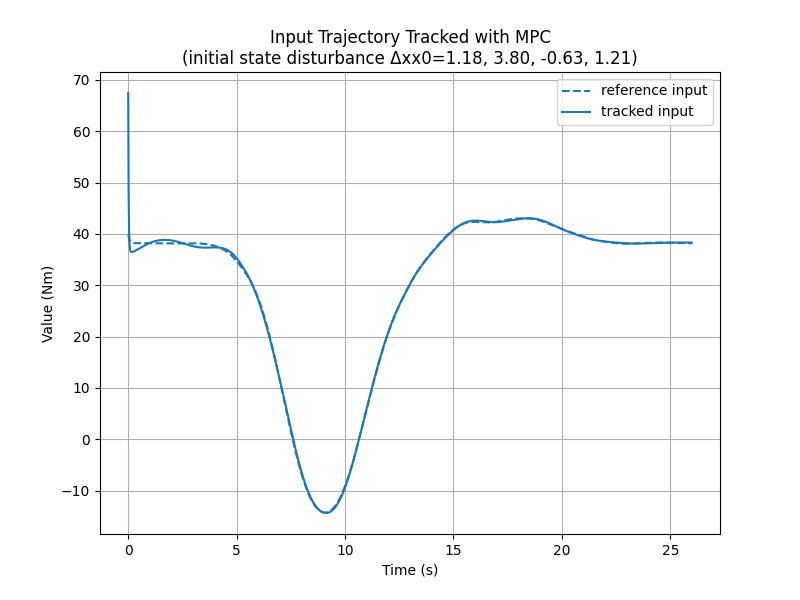
\includegraphics[width=0.9\textwidth]{input_traj_MPC__dist1_T4.png}
    \caption{Input trajectories tracked with MPC and smaller disturbance}
    \label{fig:enter-label}
\end{figure}
\begin{figure}[H]
    \centering
    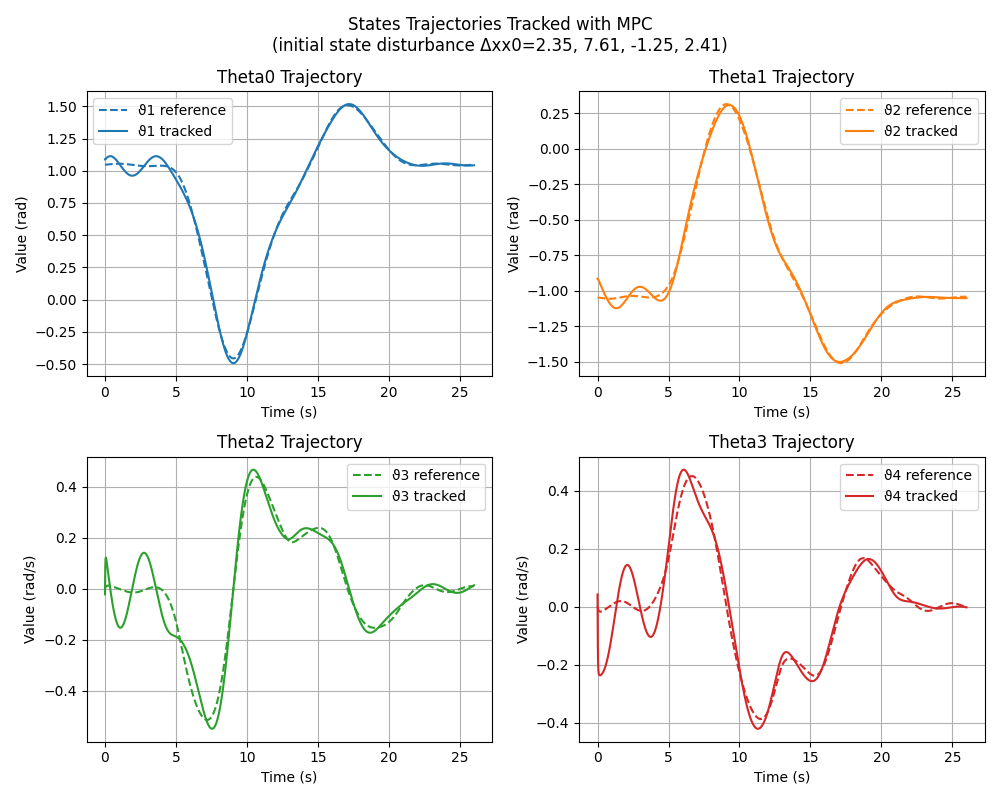
\includegraphics[width=0.9\textwidth]{State_traj_MPC_dist2_T4.png}
    \caption{States trajectories tracked with MPC and bigger disturbance}
    \label{fig:enter-label}
\end{figure}
\begin{figure}[H]
    \centering
    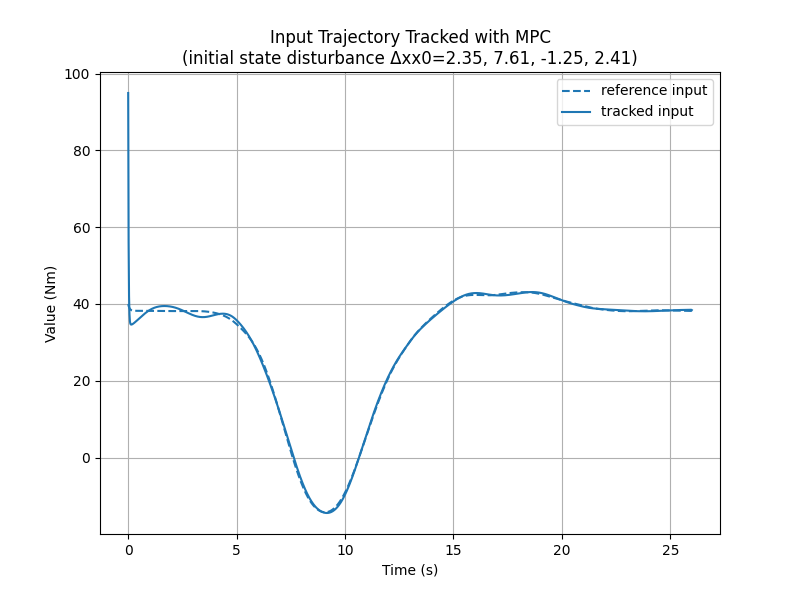
\includegraphics[width=0.9\textwidth]{Input_traj_MPC_dist2_T4.png}
    \caption{Input trajectories tracked with MPC and bigger disturbance}
    \label{fig:enter-label}
\end{figure}

\begin{figure}[H]
    \centering
    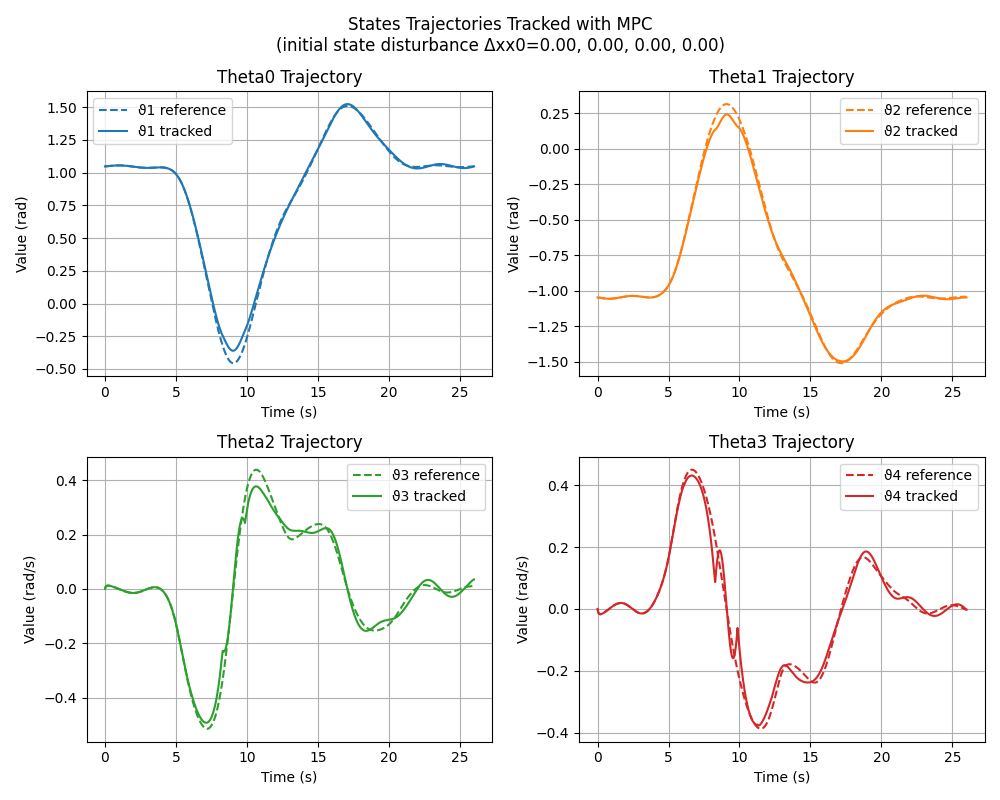
\includegraphics[width=0.8\textwidth]{State_tra_MPC_AD_T4.png}
    \caption{States trajectories tracked with MPC and no disturbance, but with input saturation}
    \label{fig:enter-label}
\end{figure}
\begin{figure}[H]
    \centering
    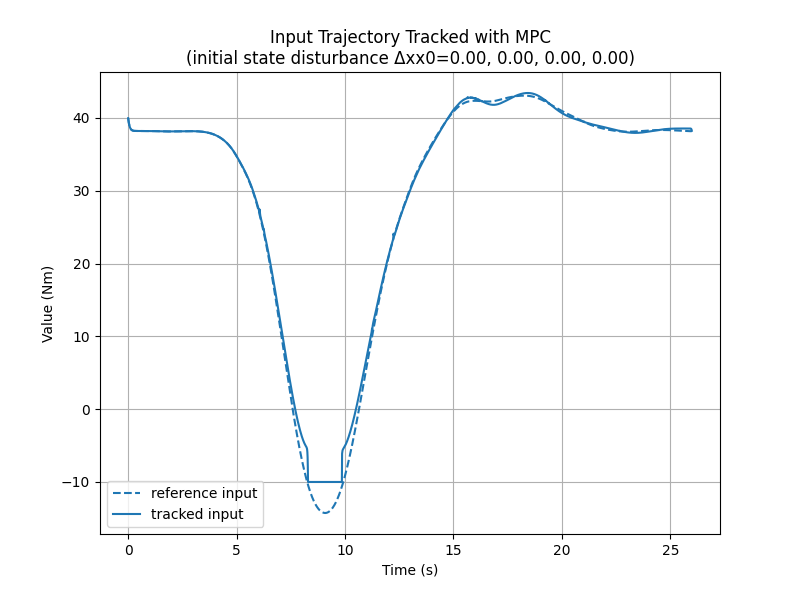
\includegraphics[width=0.8\textwidth]{Input_traj_MPC_AD_T4.png}
    \caption{Input trajectories tracked with MPC and no disturbance, but with input saturation}
    \label{fig:enter-label}
\end{figure}
\begin{figure}[H]
    \centering
    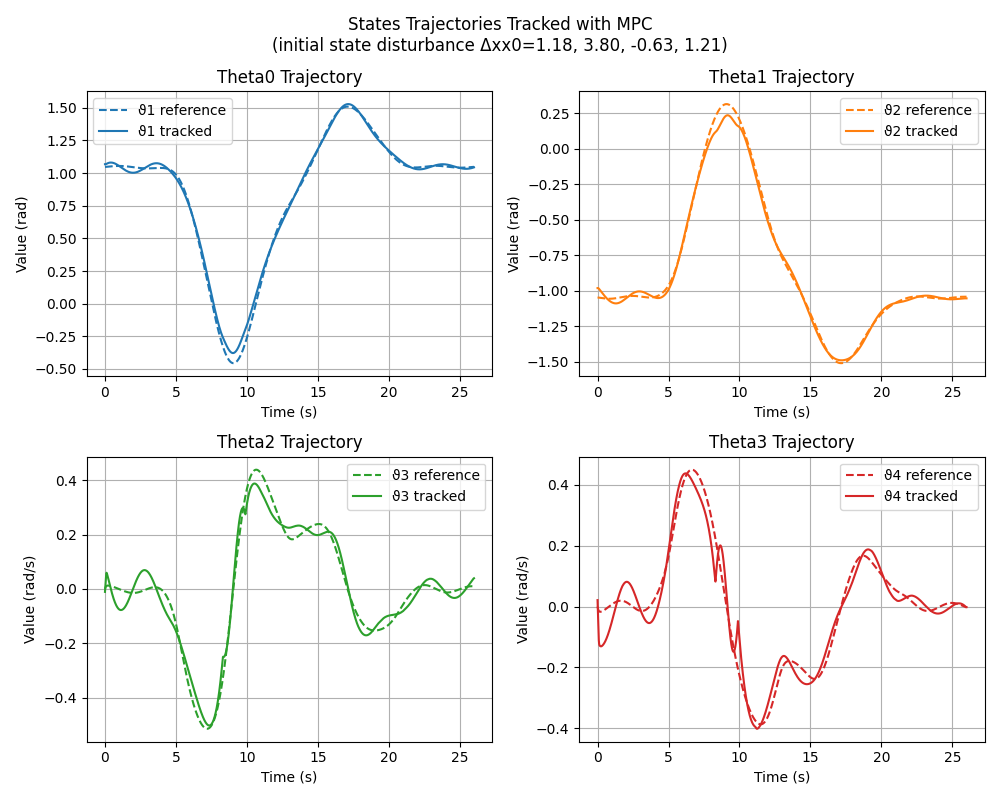
\includegraphics[width=0.8\textwidth]{State_traj_MPC_AD1_T4.png}
    \caption{States trajectories tracked with MPC and smaller disturbance, with input saturation}
    \label{fig:enter-label}
\end{figure}
\begin{figure}[H]
    \centering
    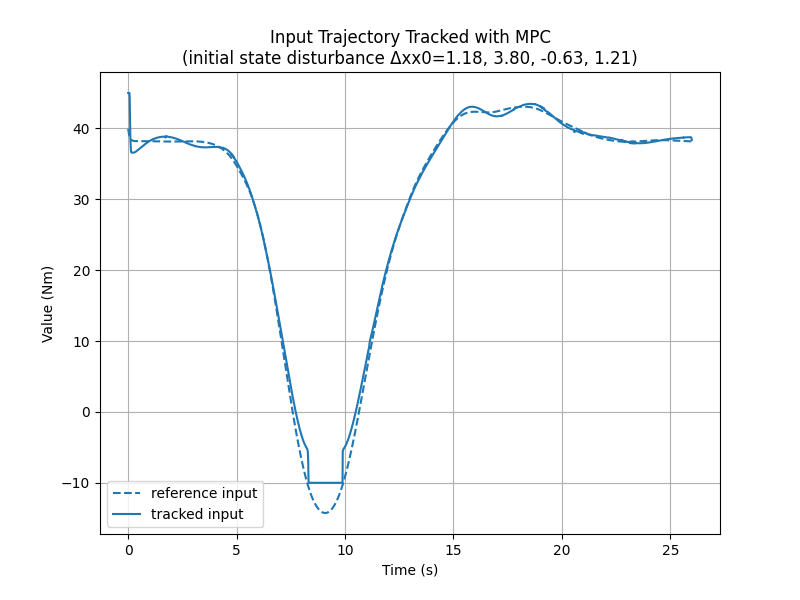
\includegraphics[width=0.8\textwidth]{Input_traj_MPC_AD1_T4.png}
    \caption{Input trajectories tracked with MPC and smaller disturbance, with input saturation}
    \label{fig:enter-label}
\end{figure}
\begin{figure}[H]
    \centering
    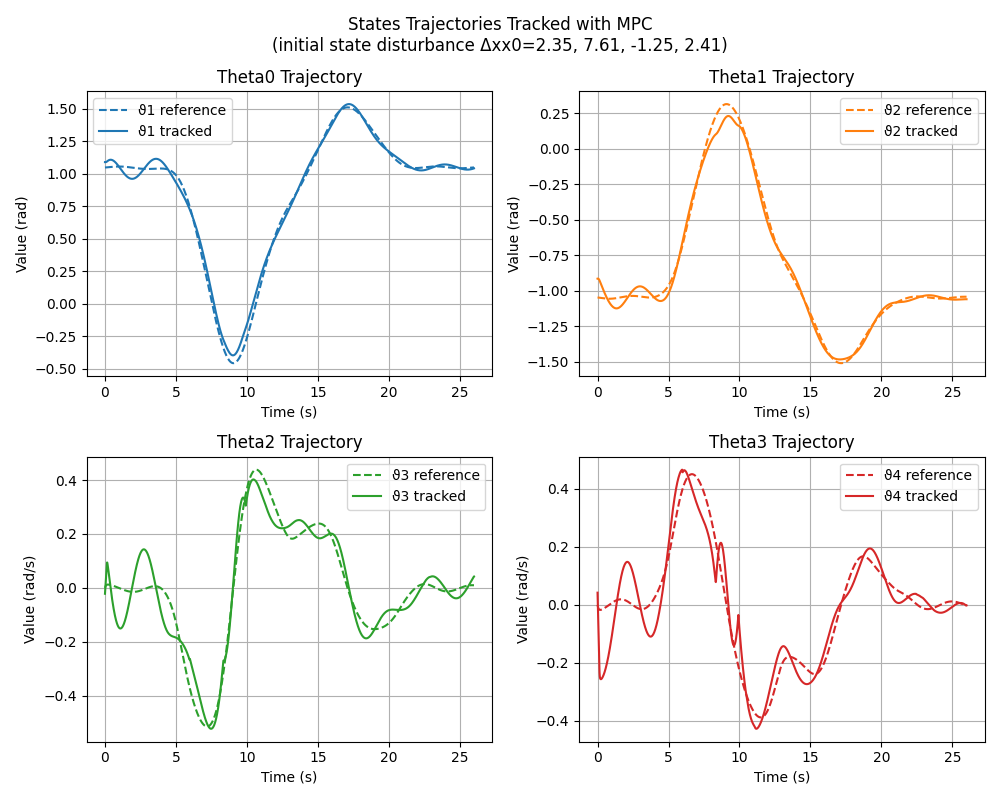
\includegraphics[width=0.8\textwidth]{state_traj_MPC_AD2_T4.png}
    \caption{States trajectories tracked with MPC and bigger disturbance, with input saturation}
    \label{fig:enter-label}
\end{figure}
\begin{figure}[H]
    \centering
    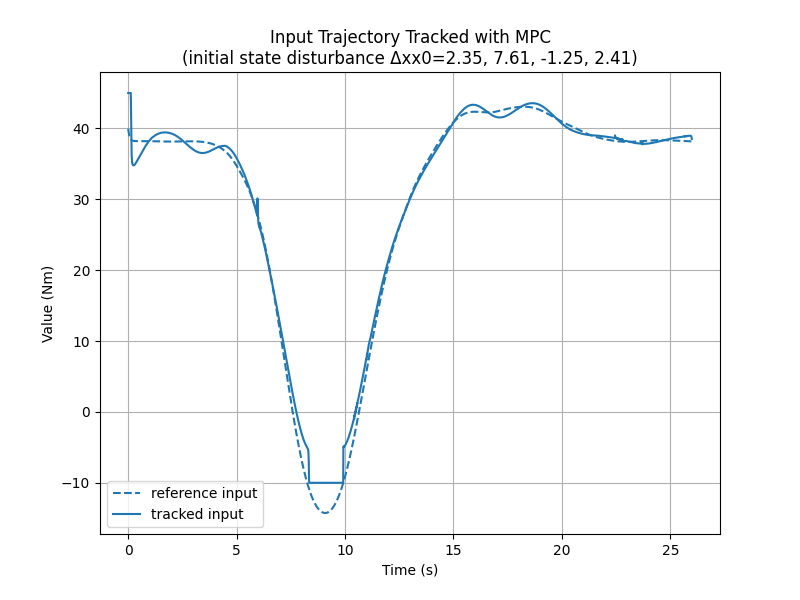
\includegraphics[width=0.8\textwidth]{input_traj_MPC_AD2_T4.png}
    \caption{Input trajectories tracked with MPC and bigger disturbance, with input saturation}
    \label{fig:enter-label}
\end{figure}

\begin{figure}[H]
    \centering
    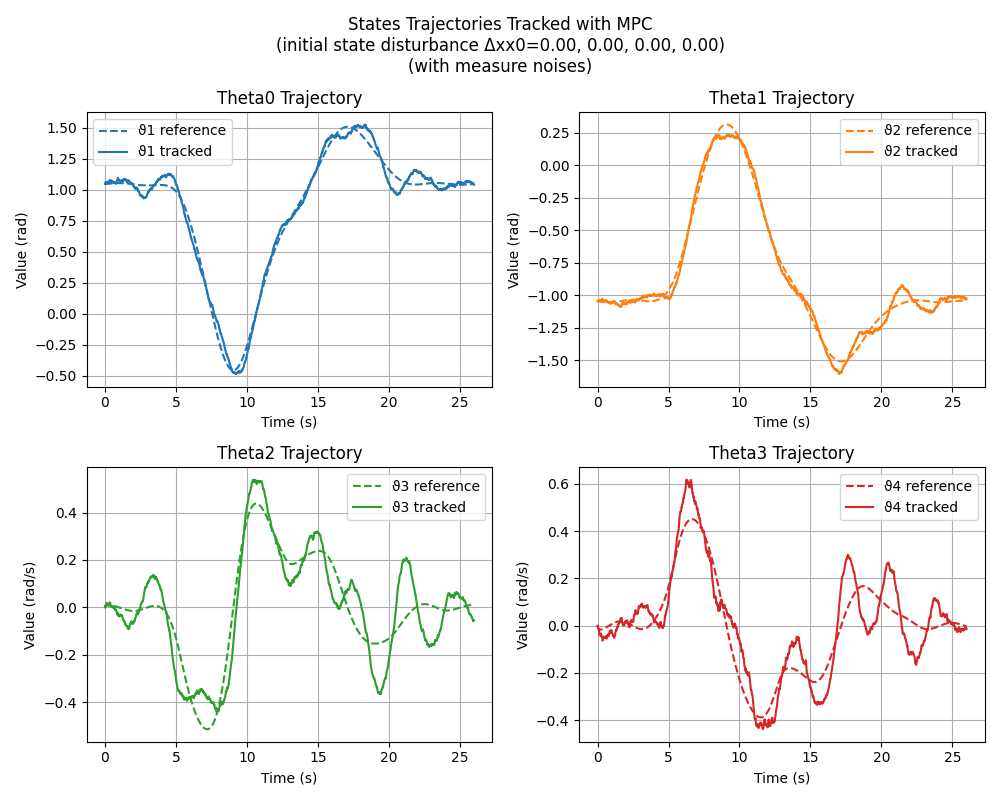
\includegraphics[width=0.8\textwidth]{state_traj_mpc_mn.png}
    \caption{States trajectories tracked with MPC and no disturbance, but with measure noise}
    \label{fig:enter-label}
\end{figure}
\begin{figure}[H]
    \centering
    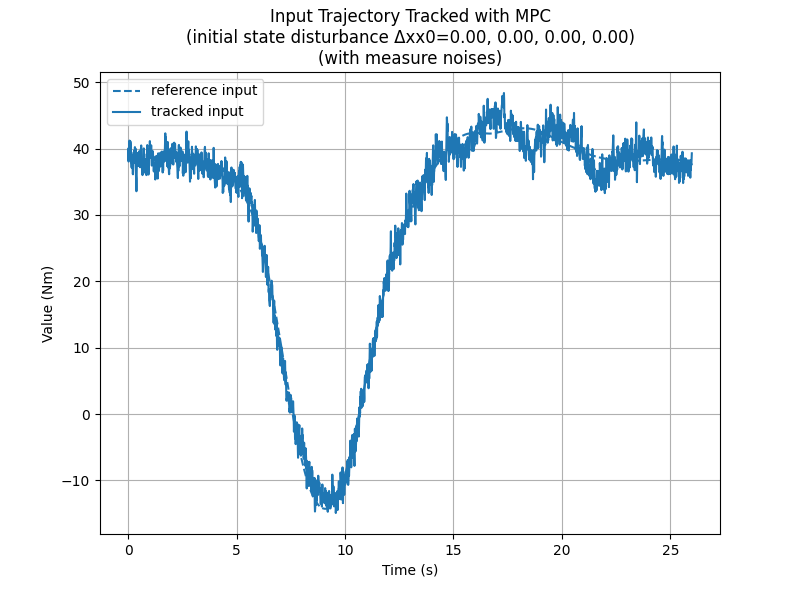
\includegraphics[width=0.8\textwidth]{input_mpc_mn.png}
    \caption{Input trajectories tracked with MPC and no disturbance, but with measure noise}
    \label{fig:enter-label}
\end{figure}
\begin{figure}[H]
    \centering
    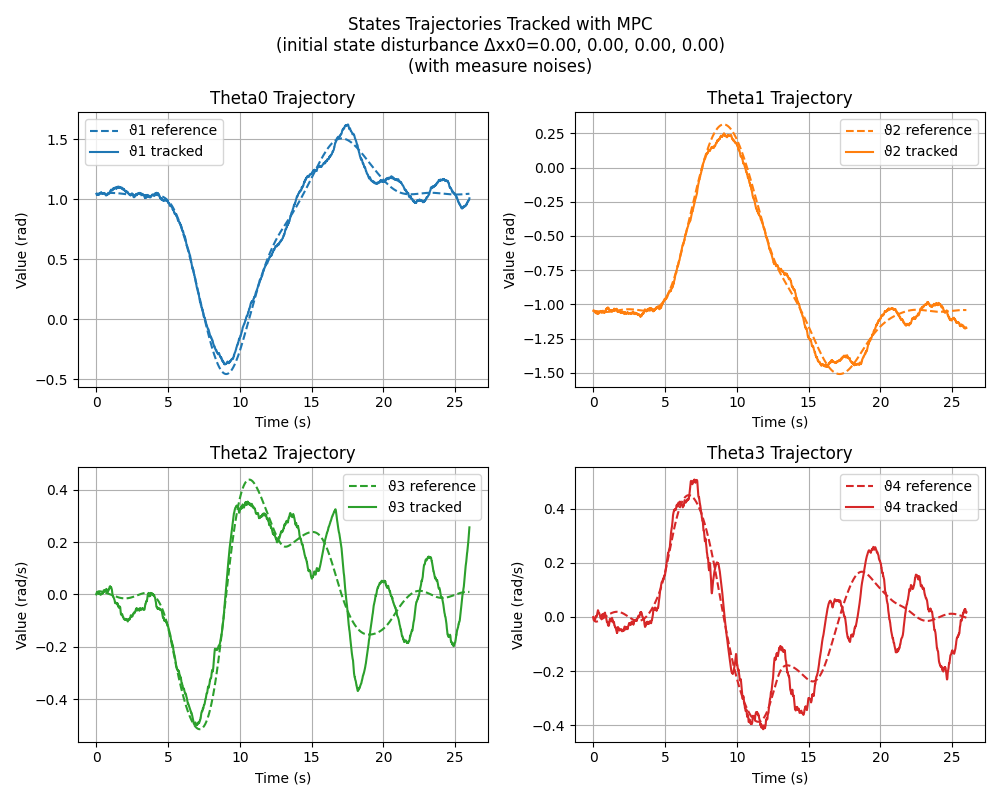
\includegraphics[width=0.8\textwidth]{state_traj_MPC_mnac.png}
    \caption{States trajectories tracked with MPC and no disturbance, with both input saturation and measure noise}
    \label{fig:enter-label}
\end{figure}
\begin{figure}[H]
    \centering
    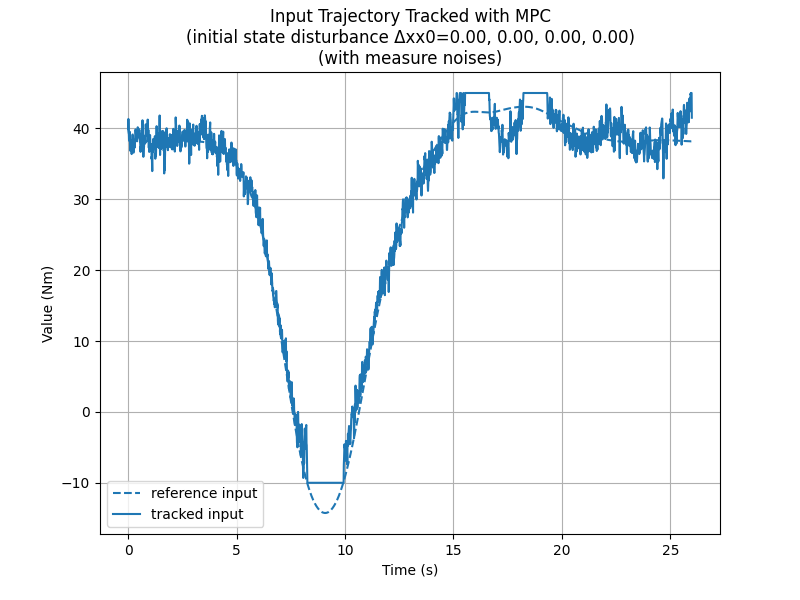
\includegraphics[width=0.8\textwidth]{input_MPC_mnac.png}
    \caption{Input trajectories tracked with MPC and no disturbance, with both input saturation and measure noise}
    \label{fig:enter-label}
\end{figure}

\clearpage

\section{Conclusions}
\begin{justify}
    {Chapter Four has examined trajectory tracking via MPC, highlighting the critical role of disturbances presence. Through an in-depth analysis of the methods and functions we described, this chapter has demonstrated how the trajectory tracking is possible and robust despite the various types of disturbance. In particular we applied firstly some initial noises and then we tried to see what would happen combining measure noises and an additional constraints, that in our case was an imput saturation. In the end, we were able to see that our MPC controller was robust enough to follow the trajectory in a satisfying way.}
\end{justify}

\chapter{Task 5 - Animation}
\section{Task description}
\begin{flushleft}
    {In this final task we have to produce a simple animation of the robot executing Task 3.}
\end{flushleft}
\begin{figure}[H]
    \centering
    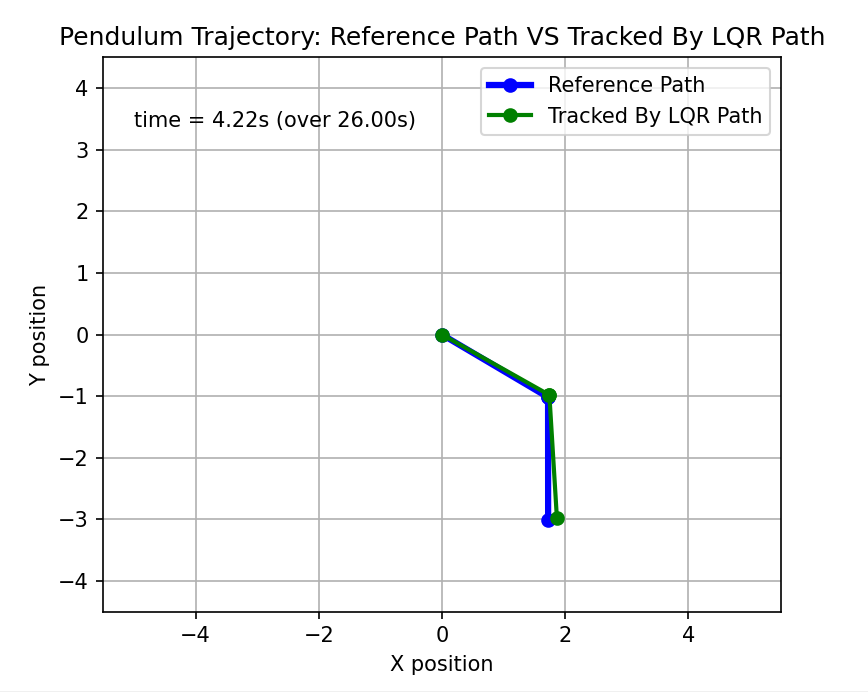
\includegraphics[width=0.8\textwidth]{Screenshot 2025-01-23 191508.png}
    \caption{first frame}
    \label{fig:enter-label}
\end{figure}
\begin{figure}[H]
    \centering
    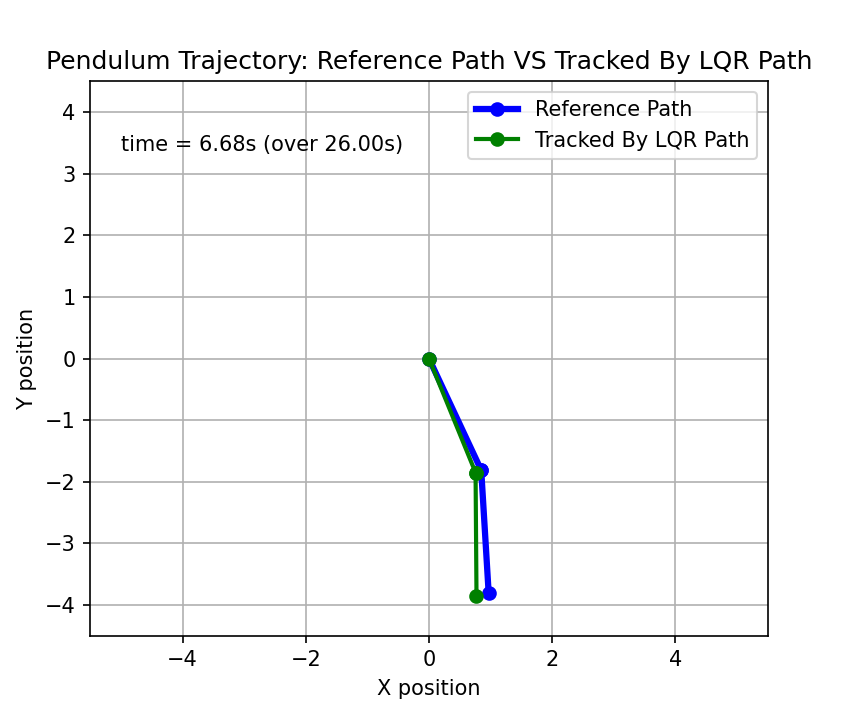
\includegraphics[width=0.8\textwidth]{Screenshot 2025-01-23 191426.png}
    \caption{second frame}
    \label{fig:enter-label}
\end{figure}
\begin{figure}[H]
    \centering
    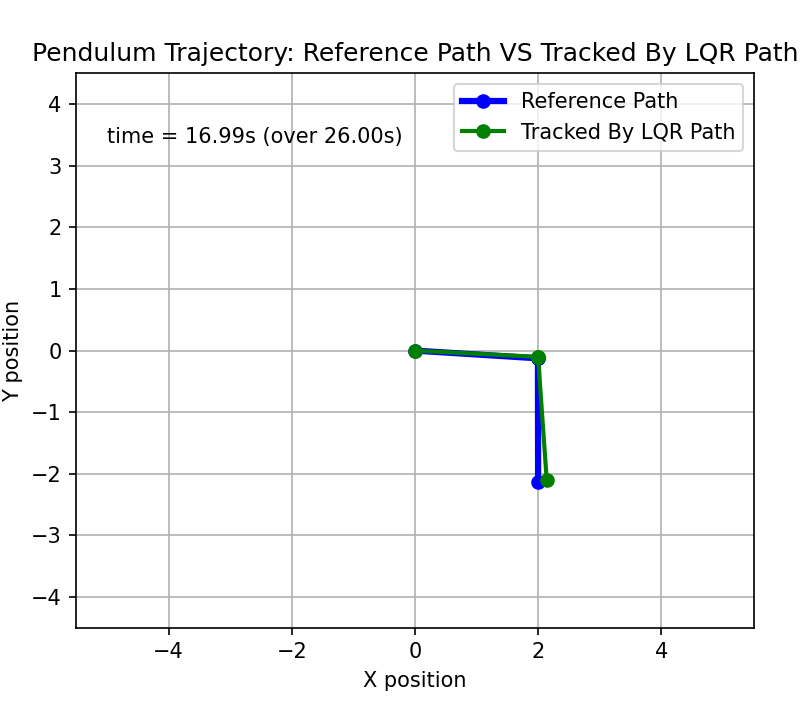
\includegraphics[width=0.75\textwidth]{Screenshot 2025-01-23 191444.png}
    \caption{third frame}
    \label{fig:enter-label}
\end{figure}



%%%%%%%%%% Conclusions %%%%%%%%%%
\chapter*{Conclusions}
\begin{justify}
\addcontentsline{toc}{chapter}{Conclusions} 
This project successfully demonstrated the design and implementation of optimal control strategies for a flexible robotic arm. Through the completion of six distinct tasks, we explored trajectory generation, optimization, and tracking using advanced control techniques.

The Newton-like algorithm proved effective for trajectory generation, enabling optimal transitions between equilibria with rapid convergence and high accuracy. Transitioning to smooth trajectories highlighted the significance of cost matrix tuning, particularly in balancing position and velocity costs to achieve optimal trajectory adherence.

The trajectory tracking methods using LQR and MPC controllers validated their robustness and efficiency under various conditions.\\ The LQR controller exhibited strong tracking performance, maintaining stability even with disturbances and measurement noise.\\ The MPC approach, on the other hand, introduced additional flexibility by being an on-line controller and being able to handle constraints such as input saturation, demonstrating its robustness in managing complex scenarios while maintaining satisfactory trajectory tracking.

The results also emphasized the importance of noise and disturbance management in practical control systems. The comparative analysis of the two control strategies under different perturbations provided valuable insights into their respective advantages and limitations.

Finally, the produced animations allowed for an intuitive visualization of the robot's performance.

In summary, the project not only validated the theoretical framework and implementation of advanced control strategies but also highlighted the challenges and intricacies associated with the control of flexible robotic systems. The findings provide a solid foundation for further exploration and application in real-world scenarios, where precision and adaptability are critical.
\end{justify}


\end{document}